\documentclass[12pt]{article}
\usepackage{framed}
\usepackage[margin=1in]{geometry} 
\usepackage{amsmath,amsthm,amssymb,graphicx,mathtools,tikz,hyperref}
\usetikzlibrary{positioning}
\newcommand{\n}{\mathbb{N}}
\newcommand{\z}{\mathbb{Z}}
\newcommand{\q}{\mathbb{Q}}
\newcommand{\cx}{\mathbb{C}}
\newcommand{\real}{\mathbb{R}}
\newcommand{\field}{\mathbb{F}}
\newcommand{\ita}[1]{\textit{#1}}
\newcommand{\com}[2]{#1\backslash#2}
\newcommand{\oneton}{\{1,2,3,...,n\}}
\newcommand\idea[1]{\begin{gather*}#1\end{gather*}}
\newcommand\ef{\ita{f} }
\newcommand\eff{\ita{f}}
\newcommand\proofs[1]{\begin{proof}#1\end{proof}}
\newcommand\inv[1]{#1^{-1}}
\newcommand\setb[1]{\{#1\}}
\newcommand\en{\ita{n }}
\usepackage{pdfpages}
\newcommand{\vbrack}[1]{\langle #1\rangle}
\newcommand{\norm}[1]{\left\lVert#1\right\rVert}
\newcommand{\La}{\mathcal{L}}
\newcommand{\Lb}{\pazocal{L}}
\usepackage[intoc, english]{nomencl}
\makenomenclature
\usepackage[titletoc]{appendix}
\usepackage{float}
\usepackage[utf8]{inputenc}
\setlength{\arrayrulewidth}{0.3mm}
\setlength{\tabcolsep}{10pt}
\renewcommand{\arraystretch}{1.5}

\newenvironment{theorem}[2][Theorem]{\begin{trivlist}
		\item[\hskip \labelsep {\bfseries #1}\hskip \labelsep {\bfseries #2.}]}{\end{trivlist}}
\newenvironment{lemma}[2][Lemma]{\begin{trivlist}
		\item[\hskip \labelsep {\bfseries #1}\hskip \labelsep {\bfseries #2.}]}{\end{trivlist}}
\newenvironment{exercise}[2][Exercise]{\begin{trivlist}
		\item[\hskip \labelsep {\bfseries #1}\hskip \labelsep {\bfseries #2.}]}{\end{trivlist}}
\newenvironment{reflection}[2][Reflection]{\begin{trivlist}
		\item[\hskip \labelsep {\bfseries #1}\hskip \labelsep {\bfseries #2.}]}{\end{trivlist}}
\newenvironment{proposition}[2][Proposition]{\begin{trivlist}
		\item[\hskip \labelsep {\bfseries #1}\hskip \labelsep {\bfseries #2.}]}{\end{trivlist}}
\newenvironment{corollary}[2][Corollary]{\begin{trivlist}
		\item[\hskip \labelsep {\bfseries #1}\hskip \labelsep {\bfseries #2.}]}{\end{trivlist}}
\hypersetup{
	colorlinks = true,
	linkcolor=blue,
	citecolor=blue
}
\begin{document}
	\date{} 
	\title{\textbf{Spacecraft Launch Vehicle Attitude Control System Design}}
	\author{Jyot Buch, Alex Hayes, Sepehr Seyedi\\ \\Group 14 : AEM 8421 : Robust Multivariable Control Systems} 
	\maketitle
	
	%%%%%%%%%%%%%%%%%%%%%%%
	\section*{Abstract}
	The launch vehicle attitude control system design is an extremely complex process requiring many years of research and development. Role of a attitude control design engineer is to design a control system that satisfies controllability, stability, transient response, GNC feedback loop schedule, etc. This project involves study of a spacecraft launch vehicle attitude control problem. Several control design objectives of a reduced order launch vehicle (LV) are explored by understanding and applying robust control concepts. Fundamental trade off between performance and robustness will be studied in this project. Most of the discussion in this paper is based on derivation of a model and explanation provided in reference \cite{cite1}. MATLAB code for this project is attached in appendix [\ref{appendix}] for reference.
	\clearpage
	%%%%%%%%%%%%%%%%%%%%%%%
	\tableofcontents
	\clearpage
	
	%%%%%%%%%%%%%%%%%%%%%%%
	\printnomenclature
	
	%%%%%%%%%%%%%%%%%%%%%%%
	\section{Dynamics}
	The nonlinear dynamics of the spacecraft launch vehicle were derived using Euler's equations of motion in \cite{cite1} under the rigid body assumption. 
	\begin{figure}[!h]
		\centering
		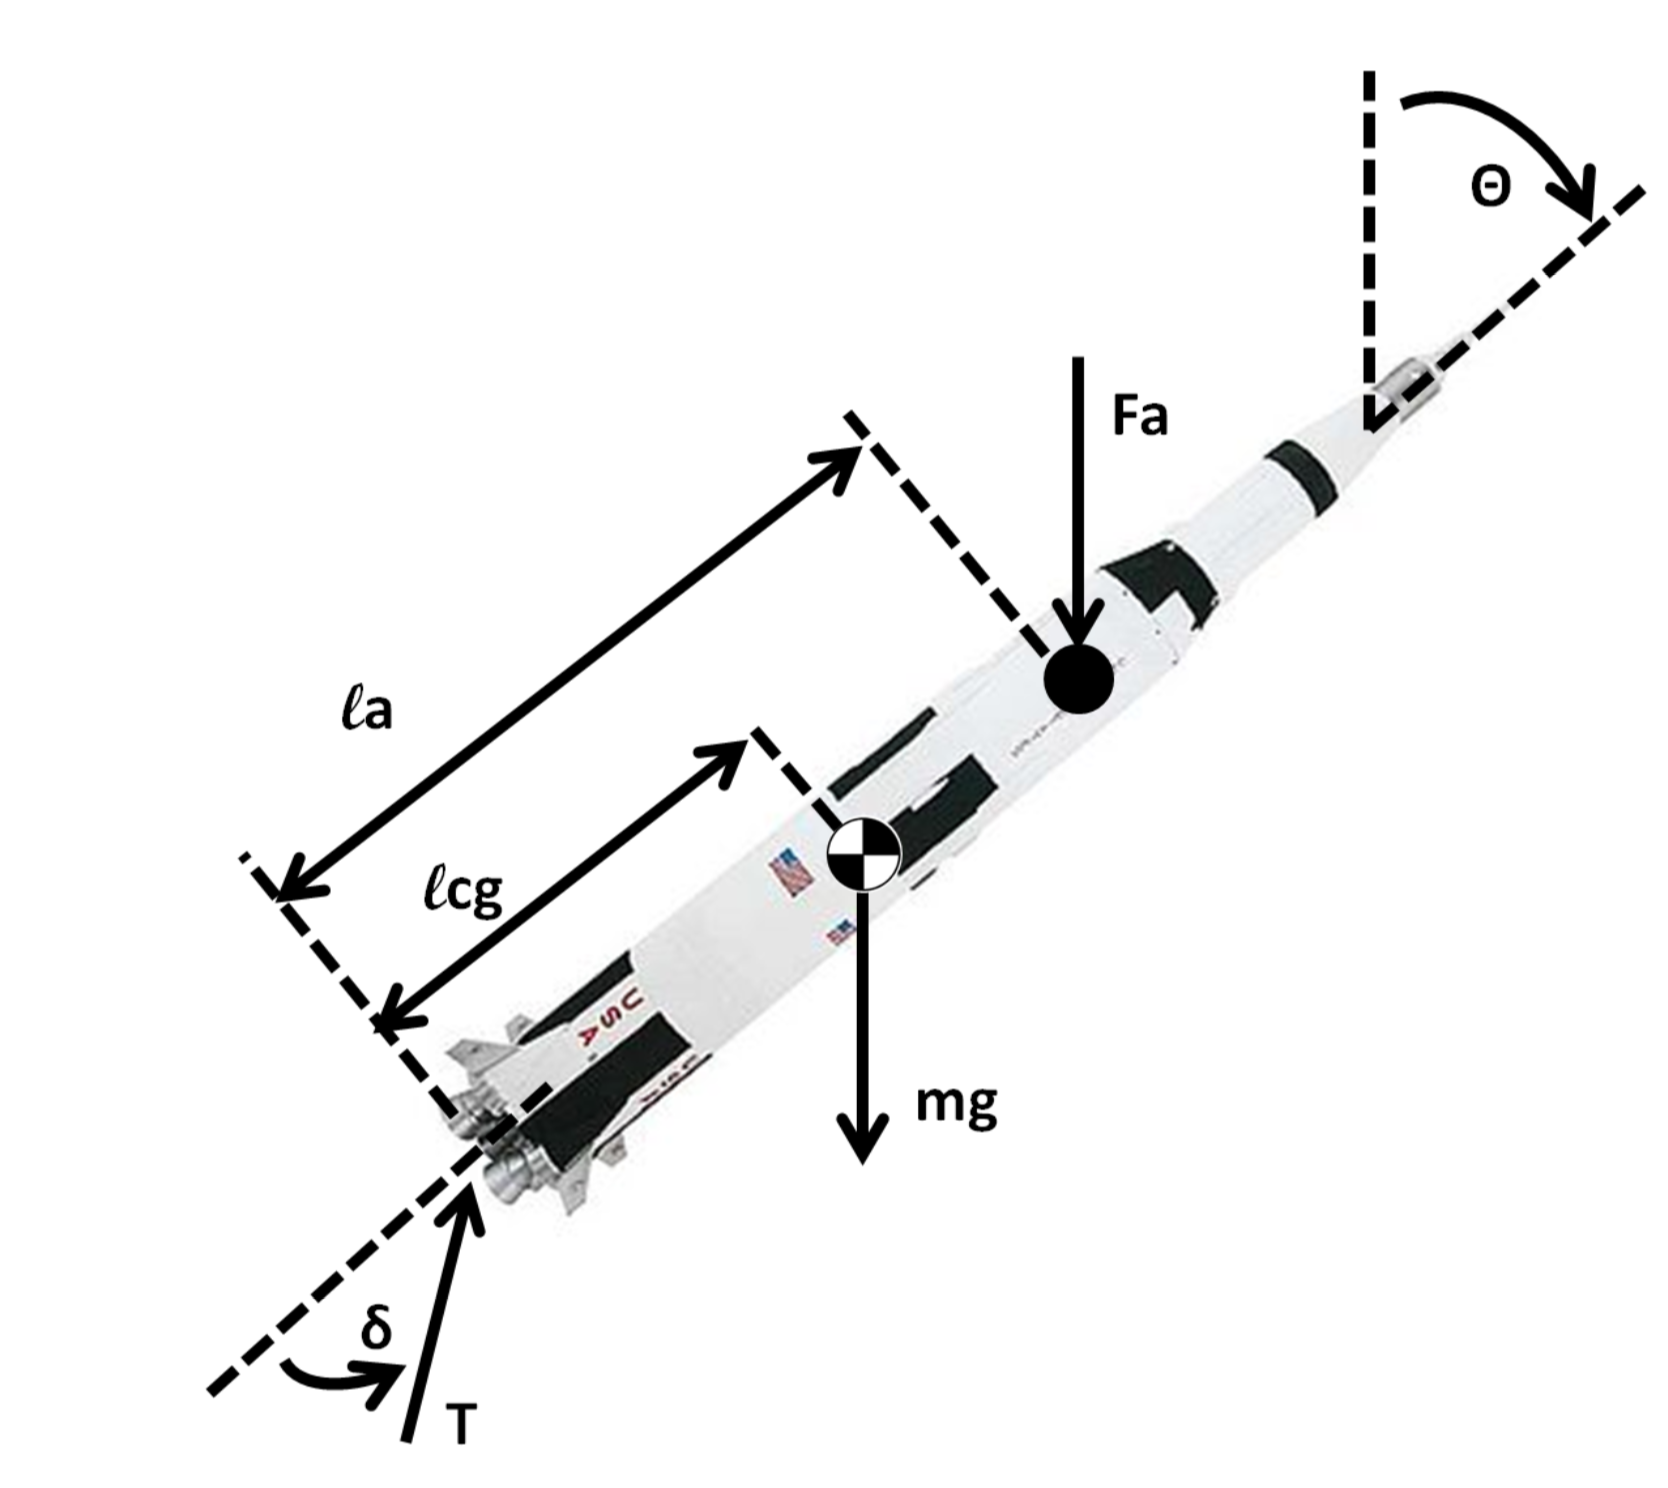
\includegraphics[width=0.6\linewidth]{Rocket}
		\caption{Rocket Attitude Free Body Diagram}
		\label{fig:rocket}
	\end{figure}
	In this work, linearized time invariant control oriented model for attitude dynamics is used for analysis. Attitude of the launch vehicle is defined by its orientation in space. Here, $\theta$ is attitude angle, $\dot{\theta}$ is angular rate, and $\delta$ is the control input related to gimbal angle or an engine deflection angle. 
	%%%%%%%%%%%%%%%%%%%%%%%
	
	%%%%%%%%%%%%%%%%%%%%%%%
	\subsection{LTI State Space Model}
	\label{ss}
	In this section, reduced order spacecraft launch vehicle attitude model is revisited \cite{cite1}. This Multi-Input Multi-Output (MIMO) model has 3 inputs and 2 outputs. The general LTI state space can be written as,
	\begin{equation}
	\label{eq1}
	\begin{split}
	\dot{\textbf{x}}&= A\textbf{x} + B\textbf{u}\\
	\textbf{y} &= C\textbf{x} + D\textbf{u}
	\end{split}
	\end{equation}
	\noindent State vector including sensor dynamics $\theta_{PG}$ and $\theta_{RG}$ is defined as, 
	\begin{equation}
	\begin{split}
	\textbf{x} = \begin{bmatrix}
	x_1 &
	x_2 &
	x_3 &
	x_4 &
	x_5
	\end{bmatrix}^{T} = \begin{bmatrix}
	\theta &
	\dot{\theta} &
	\theta_{PG} &
	\theta_{RG}&
	\dot{\theta}_{RG}
	\end{bmatrix}^{T}
	\end{split}
	\end{equation}
	\nomenclature{$\theta$}{Attitude Angle (rad)}
	\nomenclature{$\dot{\theta}$}{Attitude Angle Rate (rad/s)}
	\nomenclature{$\theta_{PG}$}{Position Gyro Output (rad)}
	\nomenclature{$\theta_{RG}$}{Rate Gyro Output (rad/s)}
	\nomenclature{$\dot{\theta}_{RG}$}{Derivative of Rate Gyro Output (rad/$s^2$)}
	
	\noindent The only exogenous control input is gimbal angle or attitude command $\delta$, including external  disturbance inputs as angle of attack $\alpha$ and wind gust $W_v$, the overall input vector can be written as,
	\begin{equation}
	\begin{split}
	\textbf{u} = \begin{bmatrix}
	u_1 \\ 
	u_2 \\
	u_3 \\
	\end{bmatrix} = \begin{bmatrix}
	\delta\\
	\alpha\\
	W_v\\
	\end{bmatrix}
	\end{split}
	\end{equation}
	
	\nomenclature{$\delta$}{Engine Deflection Angle or Gimbal Angle (rad)}
	\nomenclature{$\alpha$}{Angle of Attack (rad)}
	\nomenclature{$W_v$}{Lateral Velocity due to wind (ft/s)}
	
	\noindent Where, $A$, $B$, $C$ and $D$ matrices are given by,
	
	\begin{equation}
	A = \begin{bmatrix}
	0 & 1 & 0 & 0 & 0\\
	3.9848 & -0.00794 & 0 & 0 & 0\\
	25 & 0 & -25 & 0 & 0\\
	0 & 0 & 0 & 0 & 1\\
	0 & 21199.36 & 0 & -21199.36 & -116.48 %8479.7440
	\end{bmatrix}
	\end{equation}
	\begin{equation}
	B = \begin{bmatrix}
	0 & 0 & 0 \\
	-7.8235 & -9.413 & 0.00245 \\
	0 & 0 & 0 \\
	0 & 0 & 0 \\
	0 & 0 & 0 \\
	\end{bmatrix}
	\end{equation}
	\begin{equation}
	C = \begin{bmatrix}
	0 & 0 & 1 & 0 &  0\\
	0 & 0 & 0 & 1 & 0 \\
	\end{bmatrix}
	\end{equation}
	\begin{equation}
	D = 0_{2 \times 3}
	\end{equation}
	
	\subsection{Transfer Function}
	The transfer function of the state space model presented by equation \ref{eq1} is given by,
	\begin{equation}
	\begin{split}
	G(s)
	&= \left[
	\begin{array}{c | c}
	A  & B \\ \hline
	C & D
	\end{array}\right] = C(sI - A)^{-1}B + D
	\end{split}
	\end{equation}
	
	\section{Nominal Plant Analysis}
	\subsection{Open Loop Poles, Natural Frequency and Damping Ratio}
	Open loop eigenvalues, corresponding damping ratio and natural frequency were computed using MATLAB command \texttt{eig()} and \texttt{damp()} respectively, which are summarized in the following table. Results show that one of the eigenvalues has a positive real part i.e. $Re(\lambda_1) > 0$, resulting in unstable dynamics.  
	\begin{center}
		\begin{tabular}{ |p{2.8cm}|p{2.0cm}|p{2cm}|p{2.7cm}||p{4.2cm}| }
			\hline
			\multicolumn{5}{|c|}{Summary of Open Loop Poles} \\
			\hline
			Poles ($\underline{\lambda}$)  & Damping ($\zeta$) & Frequency (rad/s) & Time Constant (s) & Behavior\\
			\hline
			1.99 & -1 & 1.99 & 0.502 & Unstable\\
			-2.00 & 1 & 2.00 & 0.5 & Stable, Dominant\\
			-25 & 1 & 25 & 0.04 & Stable, Non-Dominant\\
			-58.24 + 133.4$j$ & 0.4 & 146 & 0.0172 & Fast-Oscillatory\\
			-58.24 - 133.4$j$ & 0.4 & 146 & 0.0172 & Fast-Oscillatory\\
			\hline
		\end{tabular}
	\end{center}
	
	It should be noted that, sensor dynamics (last 3 states) are relatively high frequency dynamics i.e. 25 rad/s and 146 rad/s respectively. Since these dynamics are having faster time constant in order of $10^{-2}$ s, we can ignore them for control analysis and derive the simplified $2^{nd}$ order model, which is done in section \ref{2ndordermodel}. Unstable pole at s = 1.99 has a negative damping, which justifies its unstable behavior with positive real part. 
	
	\subsection{Controllability}
	Using \texttt{ctrb(A,B)} command in MATLAB, controllability matrix $\mathcal{C}$ was computed and found to be full rank of $n$ = 5. Therefore, the system is full state controllable. Note that for controllability matrix, columns of B corresponding to disturbance were ignored. 
	\begin{equation}
	\mathcal{C}= \begin{bmatrix}
	B & AB & A^2B & A^3B & A^4B
	\end{bmatrix}
	\end{equation}
	
	\subsection{Observability}
	Using \texttt{obsv(A,B)} command in MATLAB, observability matrix $\mathcal{O}$ was computed and found to be full rank. Therefore, the system is full state observable.  
	\begin{equation}
	\mathcal{O}= \begin{bmatrix}
	C & CA & CA^2 & CA^3 & CA^4
	\end{bmatrix}^{T}
	\end{equation}
	Since, open loop system is both controllable and observable, it is the minimal realization of the system. It is worth remembering that above definition of controllability and observability provides binary answer such as whether the system is controllable/observable or not. 
	
	\subsection{Open Loop Frequency Response}
	Open Loop Frequency response of output 1 i.e. $\theta_{PG}$ to all the 3 input (1 control and 2 disturbance inputs) is shown in the Figure \ref{fig:bodeopenloop1}. Similarly, output 2 i.e. $\theta_{RG}$ to all the input frequency response is shown in \ref{fig:bodeopenloop2}.
	
	\begin{figure}[H]
		\centering
		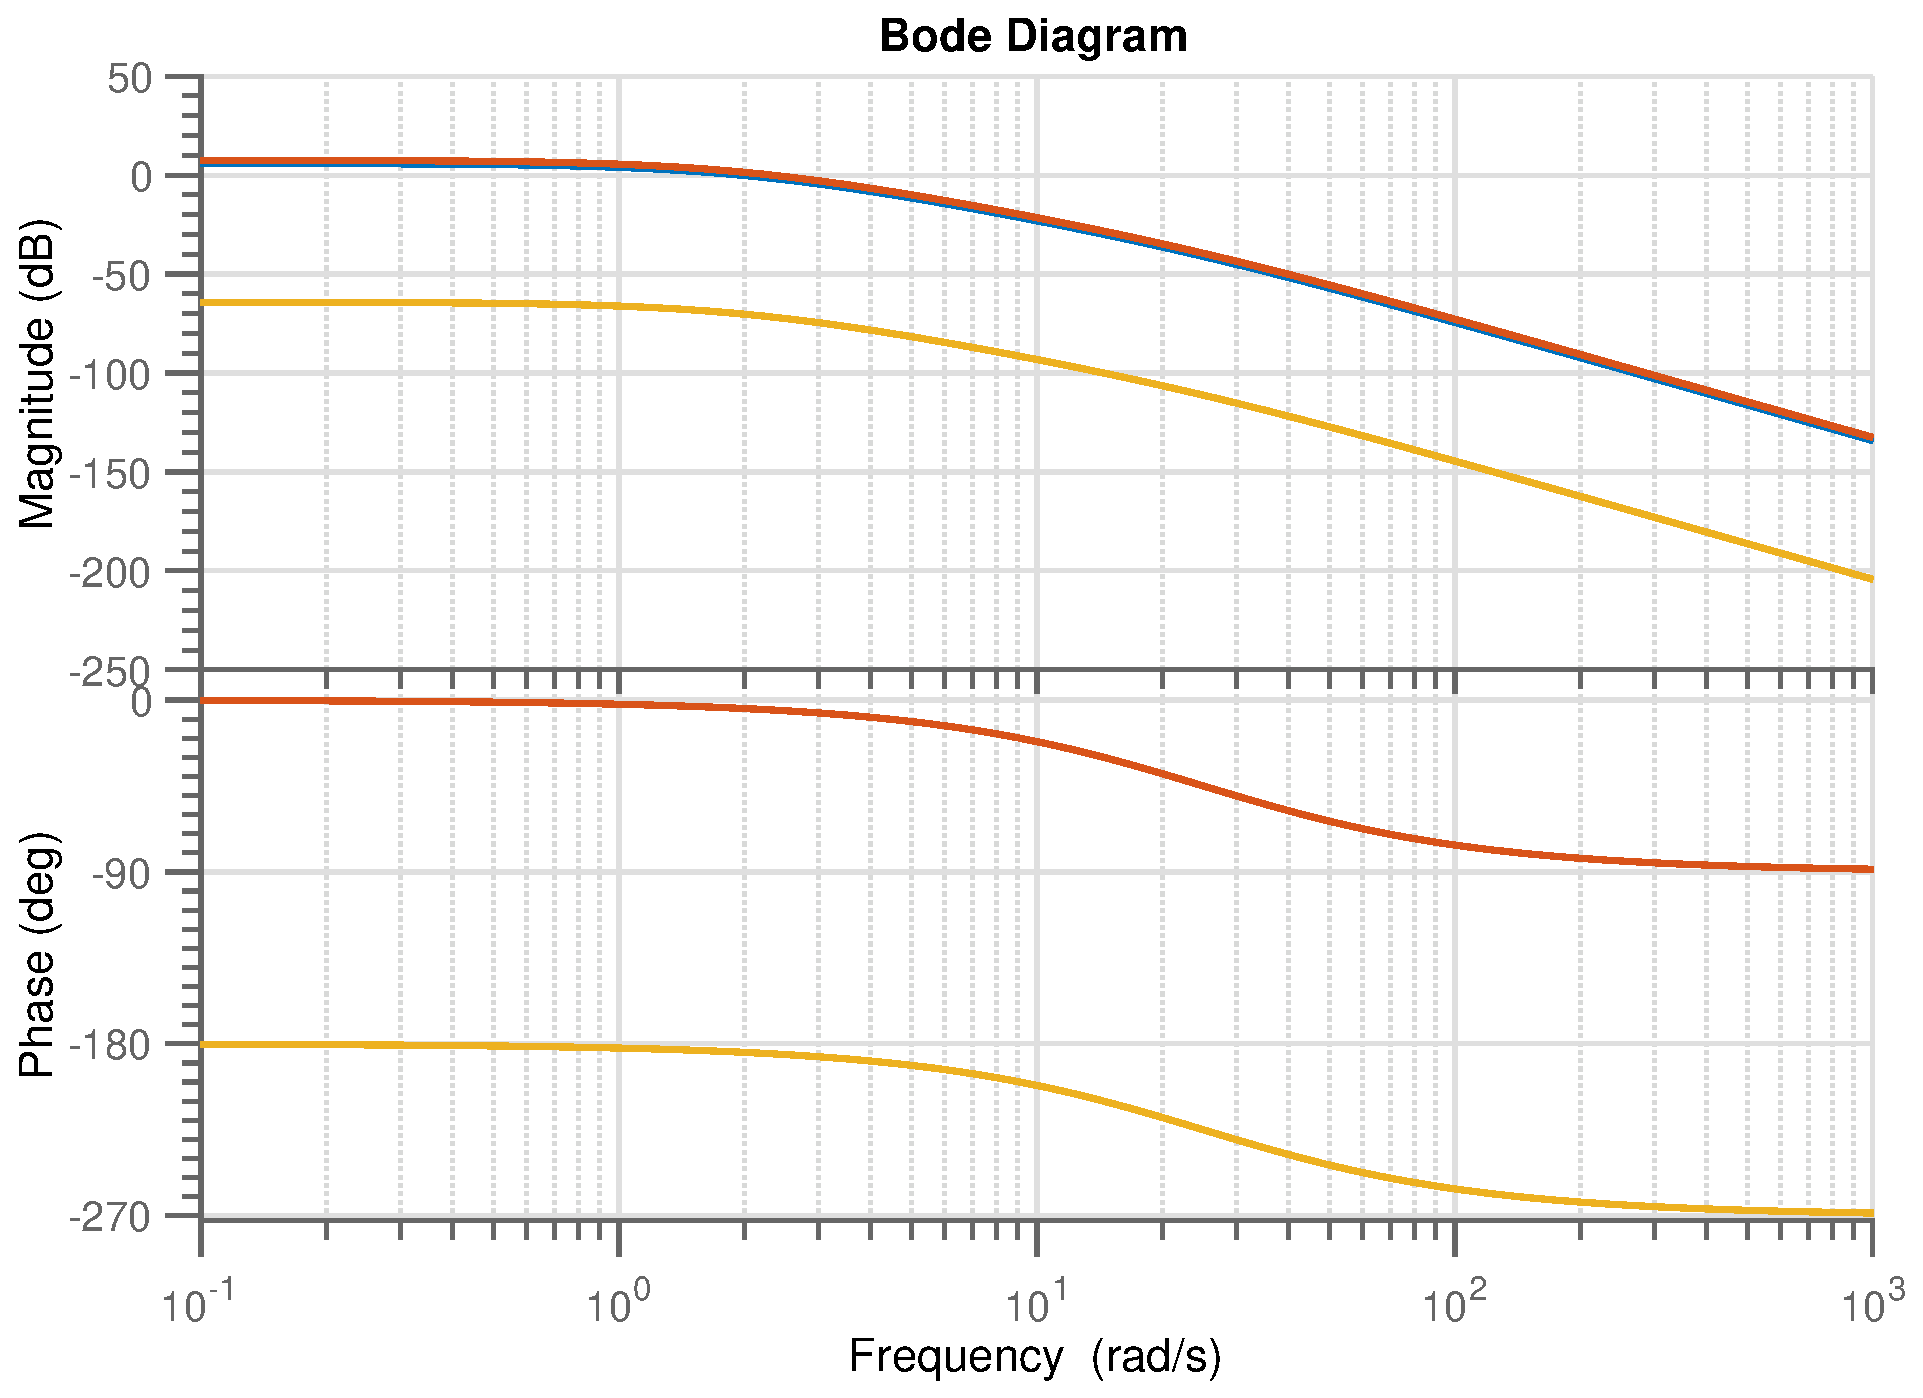
\includegraphics[width=0.8\linewidth]{bodeOpenLoop1}
		\caption{$y_1$ to $u_1$(Blue), $u_2$(Red), $u_3$(Green) Open Loop Frequency Response}
		\label{fig:bodeopenloop1}
	\end{figure}
	\begin{figure}[H]
		\centering
		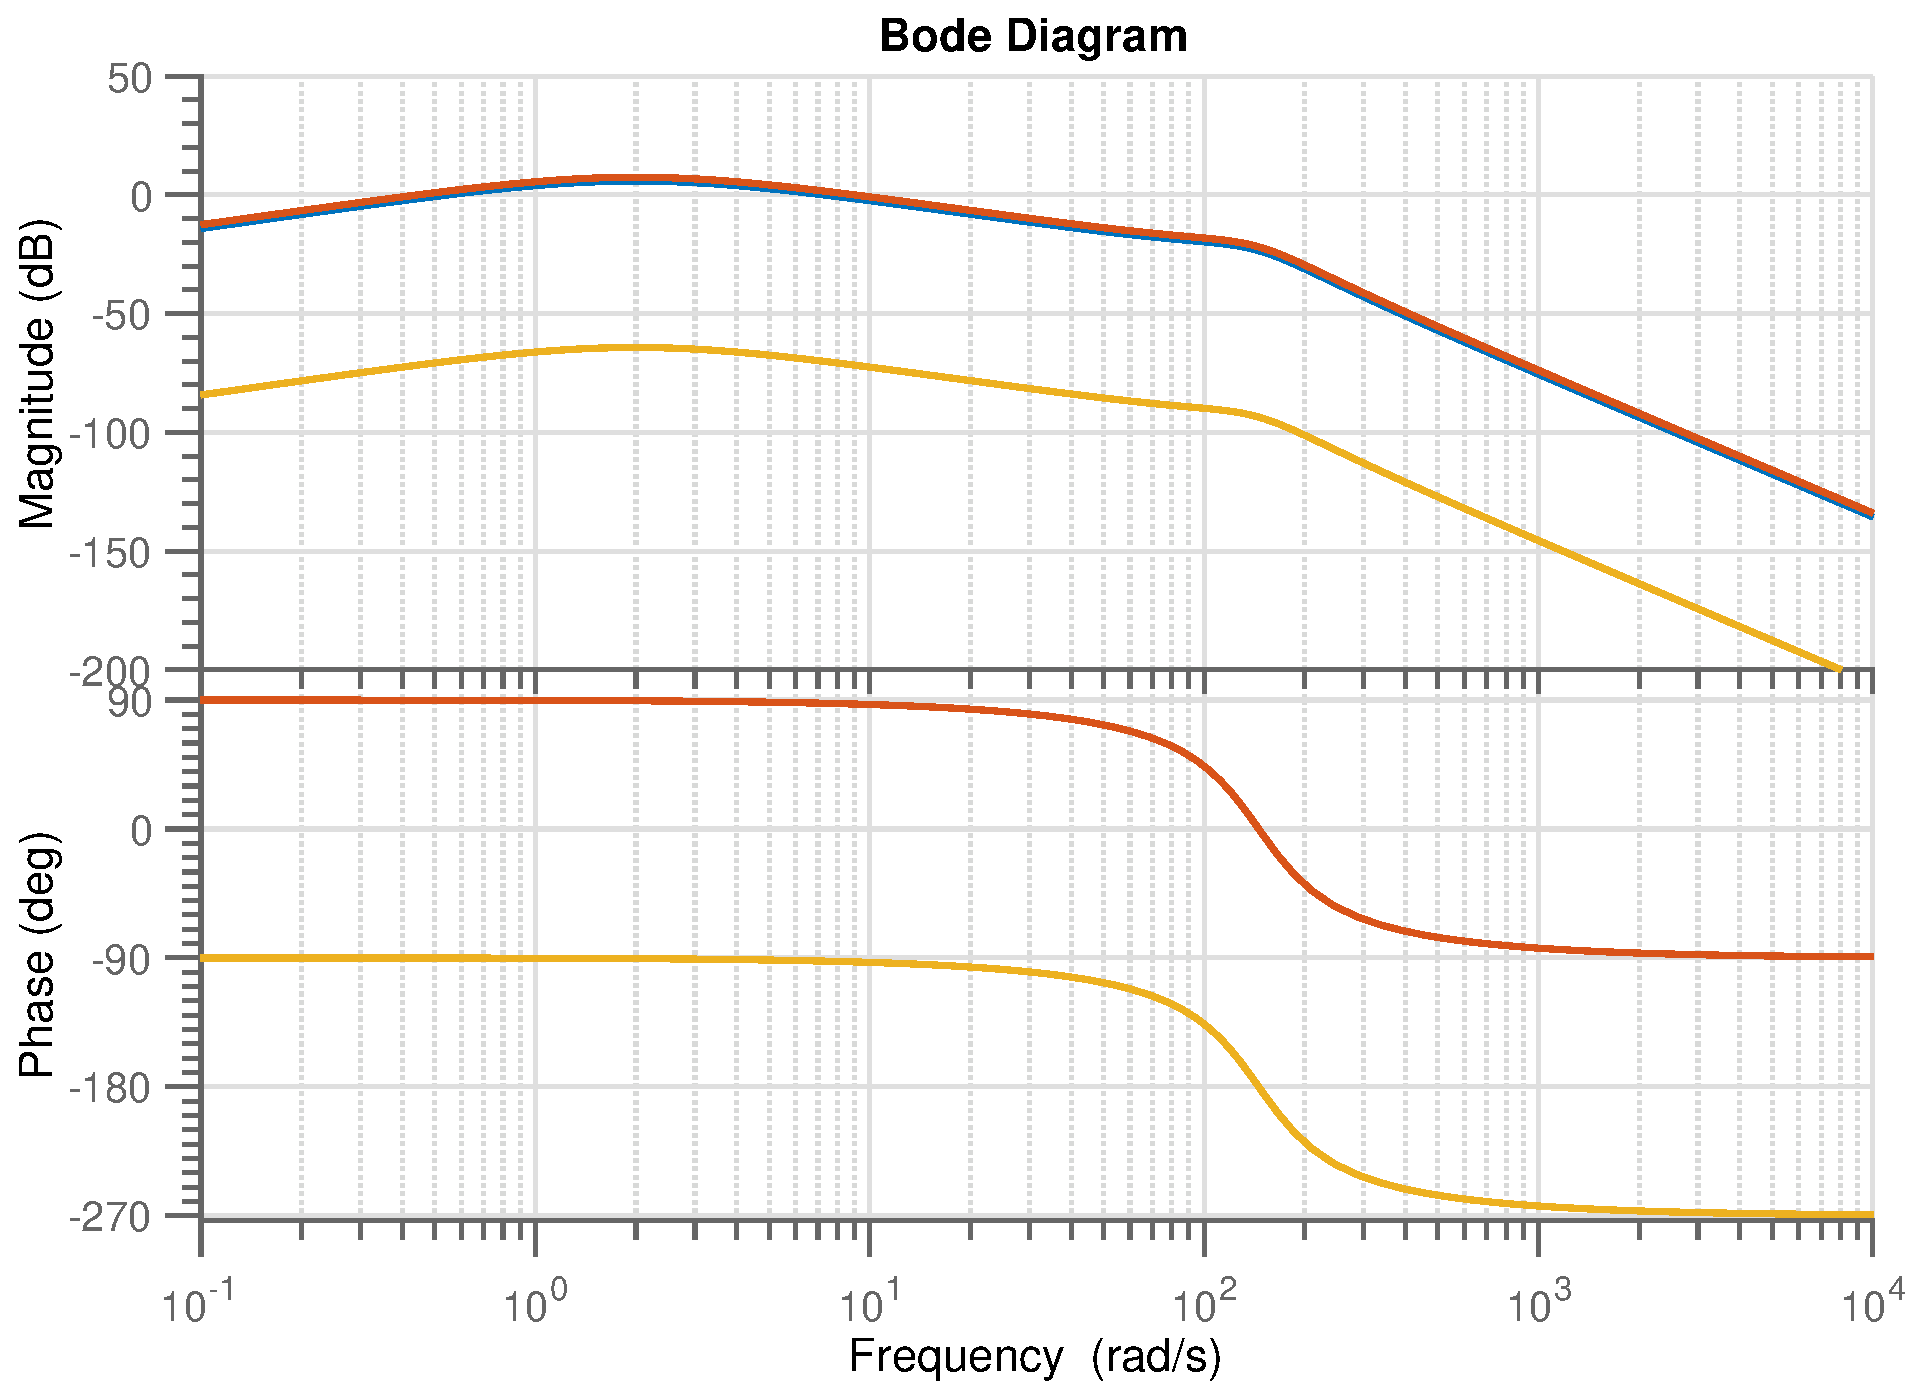
\includegraphics[width=0.8\linewidth]{bodeOpenLoop2}
		\caption{$y_2$ to $u_1$(Blue), $u_2$(Red), $u_3$(Green) Open Loop Frequency Response}
		\label{fig:bodeopenloop2}
	\end{figure}
	
	\subsection{Singular Values vs Frequency}
	Open loop singular values were computed using \texttt{svd()} function in MATLAB. It can be observed from the following singular values that largest open loop singular value $\bar{\sigma}$ = 29981 and lowest singular value $\underline{\sigma}$ = 0.7071. Further analysis is to be done in robust stability and performance section, since we need to bound the largest singular value of the overall system to ensure the robust stability. To reproduce the result shown in \cite{cite1}, the plot of singular values of the frequency response is shown in Figure \ref{fig:sigmavsfreq} using MATLAB function \texttt{sigma()}. It is observed that the peak singular value happens at approximately 1.5 rad/s with magnitude of 3.54. It is worth noticing that disturbance was also included in this analysis.
	
	%\begin{equation}
	%\sigma = \begin{bmatrix}
	%29981\\
	%35.468\\
	%2.8087\\
	%1\\
	%0.7071\\
	%\end{bmatrix}
	%\vspace{4pt}
	%\end{equation}
	\begin{figure}
		\centering
		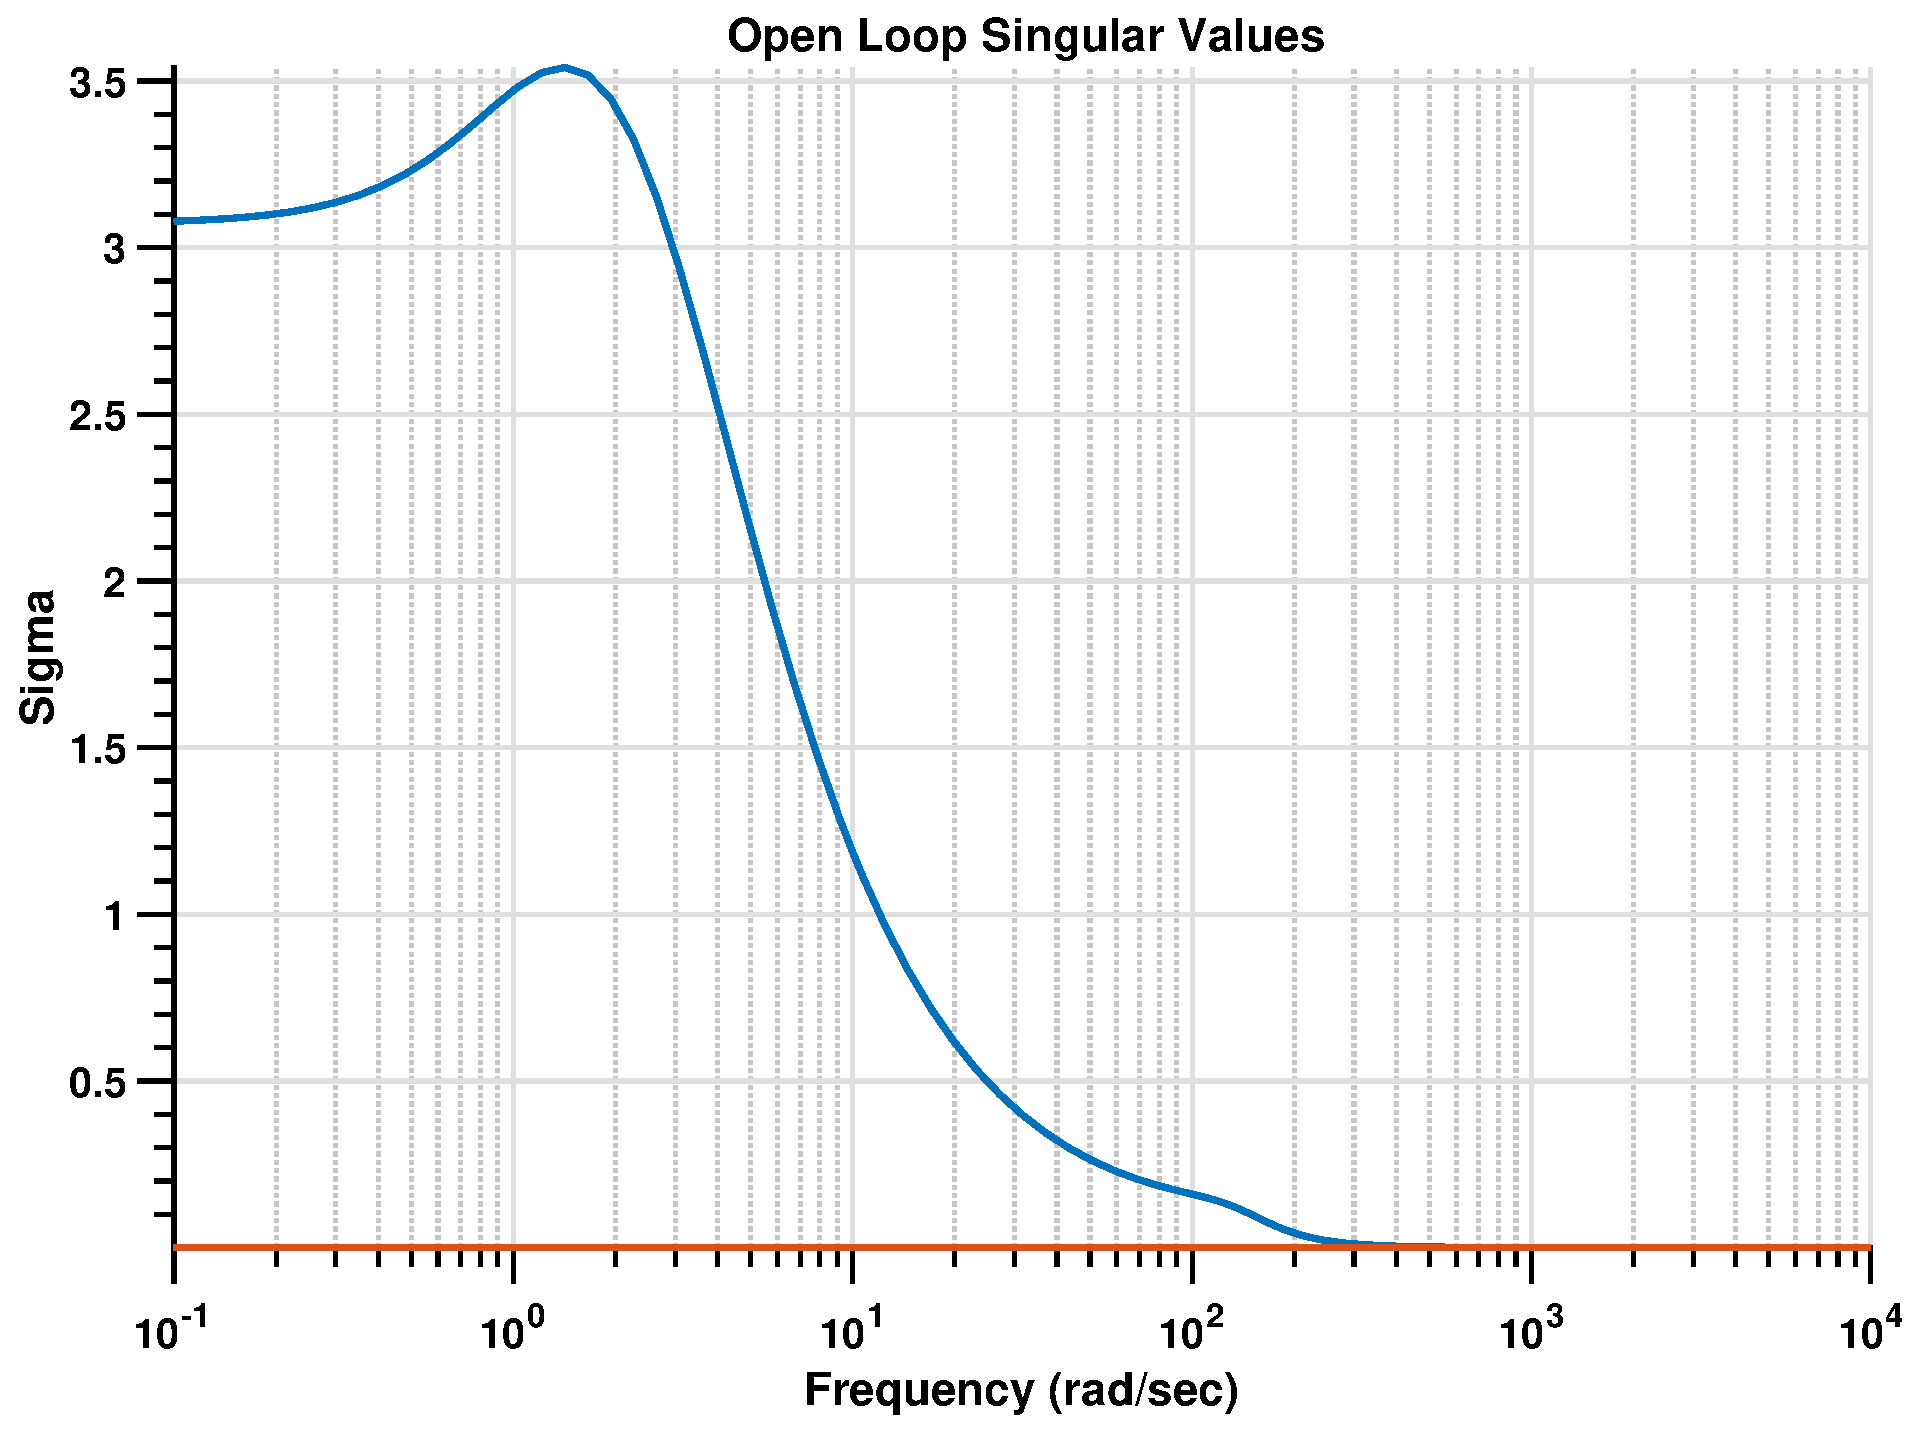
\includegraphics[width=0.8\linewidth]{SigmaVsFreq}
		\caption{Singular Values of the Frequency Response}
		\label{fig:sigmavsfreq}
	\end{figure}
	\section{Control Design}
	We now begin with the general control architecture and deign objectives followed by actual control design in MATLAB/Simulink. 
	
	\subsection{General Control Architecture}
	The generic control system is shown in Figure \ref{fig:picture1}. Actuator, Plant and Measurement Sensors are not perfect as modeled by the mathematical equations, they exhibit uncertain behavior. (Right side of the red dotted line). Lets consider the special case of the following control architecture which has a unity feedback.  \\
	\begin{figure}[!h]
		\centering
		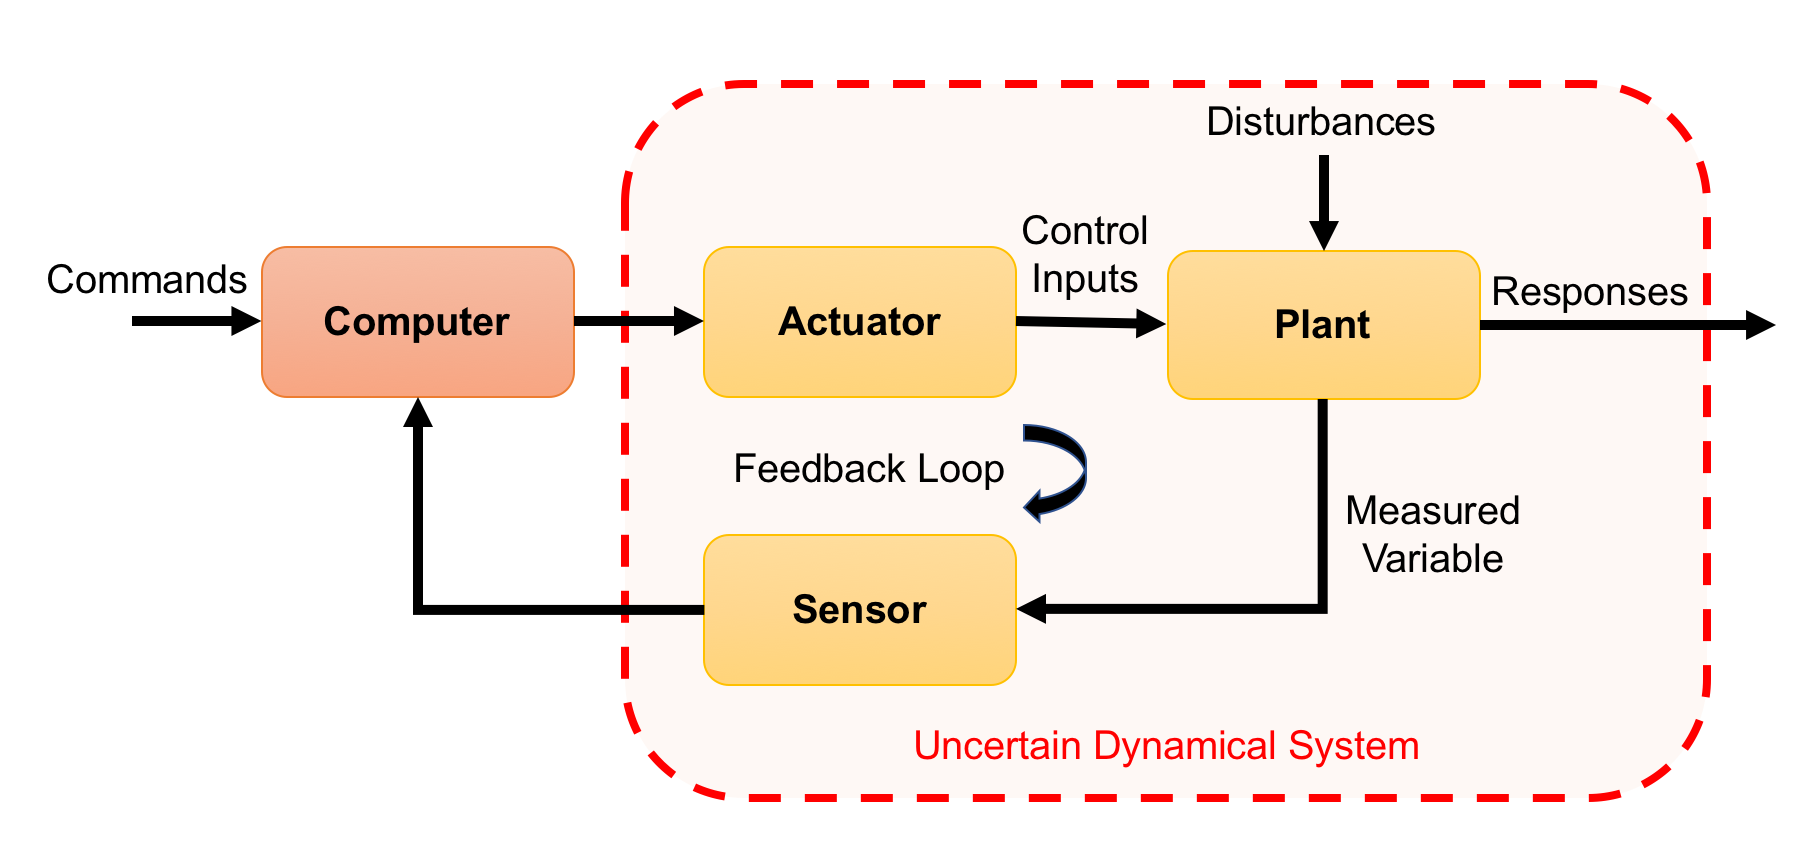
\includegraphics[width=0.8\linewidth]{img1}
		\caption{Generic Control System Layout}
		\label{fig:picture1}
	\end{figure}
	
	\noindent Here, \\
	G := MIMO Plant Transfer Function\\
	$K$ := Controller Transfer Function\\
	$r$ := Reference Signal Input\\
	$d$ := Disturbance Input\\
	$n$ := Measurement Noise\\
	
	\begin{equation}
	y = \underbrace{(I + GK)^{-1}GK}_{T}r + \underbrace{(I + GK)^{-1}}_{S}G_dd - \underbrace{(I + GK)^{-1}GK}_{T}n
	\end{equation}
	Lets define the following,
	\begin{equation*}
	\begin{split}
	G &= \text{Plant Transfer Function Matrix}\\
	K &= \text{Feedback Compensator Transfer Function}\\
	L = GK &= \text{Output Loop Transfer Function}\\
	S = (I + GK)^{-1} = (1 + L)^{-1} &= \text{Output Sensitivity Transfer Function}\\
	T = (I + GK)^{-1}GK = (1 + L)^{-1}L &= \text{Output Complementary Sensitivity function}\\
	L_I = KG &= \text{Input Loop Transfer Function}\\
	S_I = (I + KG)^{-1} = (1 + L_I)^{-1} &= \text{Input Sensitivity Transfer Function}\\
	T_I = (I + KG)^{-1}KG = (1 + L_I)^{-1}L_I &= \text{Input Complementary Sensitivity function}\\
	\text{Note that, } S + T &= I \text{ or } S_I + T_I = I
	\end{split}
	\end{equation*}
	
	\begin{figure}[H]
		\centering
		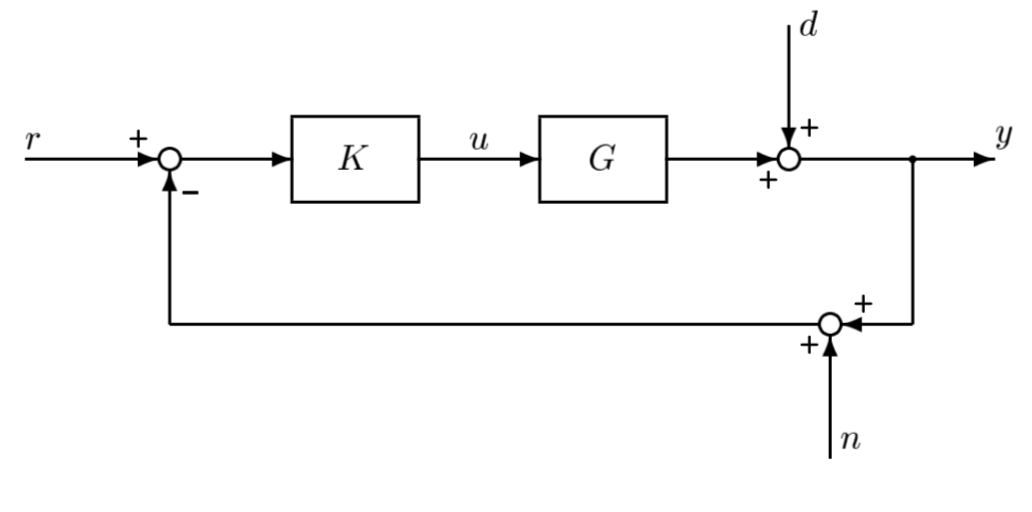
\includegraphics[width=0.7\linewidth]{fig2}
		\caption{Unity Feedback System}
		\label{fig:fig2}
	\end{figure}
	
	\noindent We have following important relationships \cite{cite3} in Laplace domain,
	\begin{equation}
	\begin{split}
	y(s) = T(s)r(s) + S(s)d(s) - T(s)n(s)\\
	u(s) = K(s)S(s)[ r(s) - n(s) - d(s)]
	\end{split}
	\end{equation}
	
	\noindent These relationships determine several closed-loop objectives as presented in \cite{cite3}, in addition to the requirement that K stabilizes G.  In what follows, we discuss some of the approximation of these in to open-loop objectives over specified frequency range.
	
	\subsection{Design Objectives}
	\noindent It is desired to have following control objectives for design considerations. 
	\begin{center}
		\noindent \begin{tabular}{ |p{8.5cm}|p{8.5cm}| }
			\hline
			\multicolumn{2}{|c|}{\textbf{Control Objectives}} \\
			\hline
			\textbf{Qualitative} & \textbf{Quantitative} \\
			\hline
			Stabilize the unstable launch vehicle dynamics & Place eigenvalues to the left half of the s-plane\\ 
			\hline
			Reduce sensitivity to disturbances & Make $\underline{\sigma}(L)$ large; for $\omega$ at which $\underline{\sigma}(L) \gg 1$\\
			\hline
			Robustness to model uncertainties & Make sure the signal norms are bounded\\
			\hline
			Noise Attenuation & Make $\bar{\sigma}(L)$ small; for $\omega$ at which $\bar{\sigma}(L) \ll 1$ \\
			\hline
			Track attitude angle reference $\theta_{ref}$ & Make $\underline{\sigma}(L)$ large; for $\omega$ at which $\underline{\sigma}(L) \gg 1$\\
			\hline
			Robust stability to an additive perturbation & Make $\bar{\sigma}(K)$ small; for $\omega$ at which $\bar{\sigma}(L) \ll 1$ \\
			\hline
			Minimize control effort & Make $\bar{\sigma}(K)$ small; for $\omega$ at which $\bar{\sigma}(L) \ll 1$ \\ \hline
		\end{tabular}
	\end{center}
	
	\noindent Where, $\underline{\sigma}(L)$ and $\bar{\sigma}(L)$ are the smallest singular value and largest singular value of loop transfer function $L$ respectively.\\
	
	\noindent Classical notion of the robustness such as gain margin $|G(jw_g)| \geq$ 6 dB, and phase margin of $\angle G(jw_c) \geq 45^o$ is desired. It is desired to have the system behavior such as low pass filter.\\
	
	\noindent In terms of time domain performance, it is desired to have, ...
	\begin{itemize}
		\item Faster rise time, in the order of 2 s or less
		\item Settling time in the order of less than 5 seconds
		\item None or minimum overshoot/undershoot
		\item With respect to maximum disturbance (i.e. High Altitude Wind $\approx$ 100 m/s, Angle of Attack $\alpha \approx$ $5-15^{o}$) no more than $5^{o}$ of overshoot in attitude angle $\theta$
		\item Adequate damping to mitigate any oscillations due to disturbance
		\item Less than 10\% steady state error in reference tracking 
	\end{itemize}
	
	\subsection{Trade-offs in MIMO feedback design}
	
	The shaping of multi-variable transfer functions is based on the idea that a satisfactory definition of gain (range of gain) for a matrix transfer function is given by the singular values of the transfer function. By multivariable transfer function shaping, therefore, we mean the shaping of singular values of appropriately specified transfer functions such as the loop transfer function or possibly one or more closed-loop transfer functions. The open-loop requirements specified in above table cannot all be satisfied simultaneously. Feedback design is therefore a trade-off over frequency of conflicting objectives. This is not always as difficult as it sounds because the frequency ranges over which the objectives are important can be quite different \cite{cite3}. For example, disturbance rejection is typically a low frequency requirement, while noise mitigation is often only relevant at higher frequencies. 
	
	\subsection{Reduced Order Model and Control Design}
	\label{2ndordermodel}
	For the purpose of control design, first a single control input system with two state variables and two outputs, both being $ \theta $ and $ \dot{\theta}$ was considered for the system shown in section \ref{ss} (See equation \ref{eq15}, which denotes $A_2$,$B_2$,$C_2$,$D_2$). As stated before, it is a valid argument to ignore the high frequency sensor dynamics for primary control design. The results will be verified in what follows with the higher order model.
	\begin{equation}
	\label{eq15}
	\begin{split}
	\frac{d}{dt}
	\begin{bmatrix}
	\theta \\ \dot{\theta}
	\end{bmatrix}
	&= \begin{bmatrix}
	0 & 1 \\
	3.9848 & -0.00794
	\end{bmatrix}\begin{bmatrix}
	\theta \\ \dot{\theta}
	\end{bmatrix} + \begin{bmatrix}
	0 \\ -7.8235
	\end{bmatrix}\delta \\
	y &= \begin{bmatrix}
	1 & 0\\
	0 & 1\\
	\end{bmatrix}\begin{bmatrix}
	\theta \\ \dot{\theta}
	\end{bmatrix}
	\end{split}
	\end{equation}
	
	\subsubsection{Proportional Control Design}
	\label{pcontrol}
	Initial approach to the control design was attempted by proportional feedback controller obtained via LQR. MATLAB command \texttt{lqr()} was used for the design. The control gains were computed by minimizing the following quadratic cost function. 
	
	\begin{equation}
	J(u) = \int_{0}^{\infty} (x^{T}Qx + u^{T}Ru) dt
	\end{equation}
	
	\noindent Where, tuning parameters such as input cost R was chosen to be 1 and state cost Q as identity matrix \texttt{eye(2)} to begin with the control design. Later, using trial and error controller gain K = [-3 -1.3] was selected to place the closed loop poles and get the desired control behavior. These gains were then plugged in to full 5 state controller and closed loop response was simulated. Thus, if the designed controller for 2 state is $K = [k_1,  k_2]$ then following controller matrix is used for full 5 state simulation in Simulink.
	
	\begin{equation}
	K_5 = \begin{bmatrix}
	k_1 & k_2\\
	0&0\\
	0&0\\
	\end{bmatrix} = \begin{bmatrix}
	-3 & -1.3 \\
	0&0\\
	0&0\\
	\end{bmatrix}
	\end{equation}
	
	\noindent Thus in summary, we first begin the design of a controller with reduced order model using 2 states i.e. $\theta$, $\dot{\theta}$ and then use the resulting control gains for the full state model by plugging them in to sensor states i.e. $\theta_{PG}$ and $\theta_{RG}$ instead of the true one. It can be seen from the Figure \ref{fig:disturbancerejectionpcontrol} that proportional feedback does well in terms of tracking 0 attitude angle (solid line) but, it does not reduce the steady state error in $\theta$ due to wind gust or angle of attack step (dashed line) disturbances, resulting in steady state offset in attitude angle. Figure \ref{fig:disturbancerejectionpcontrol} demonstrates the case when angle of attack step disturbance was applied at t = 8 s with step magnitude of $-5^{o}$. Here, negative angle of attack disturbance results in positive offset for attitude angle $\theta_{RG}$. Initial conditions of [$\theta$,$\dot{\theta}$,$\theta_{PG}$,$\theta_{RG}$,$\dot{\theta}_{RG}$] = [0.087, 0.087, 0.087, 0.087, 0] were provided to the full 5 state model to simulate the closed loop response ($0.087$ rad $\approx 5^{o}$). Figure \ref{fig:disturbancerejectionpcontrol} shows that proportional controller fails to track $\theta_{ref}$ = 0 angle in the presence of disturbance.
	
	\begin{figure}[!h]
		\centering
		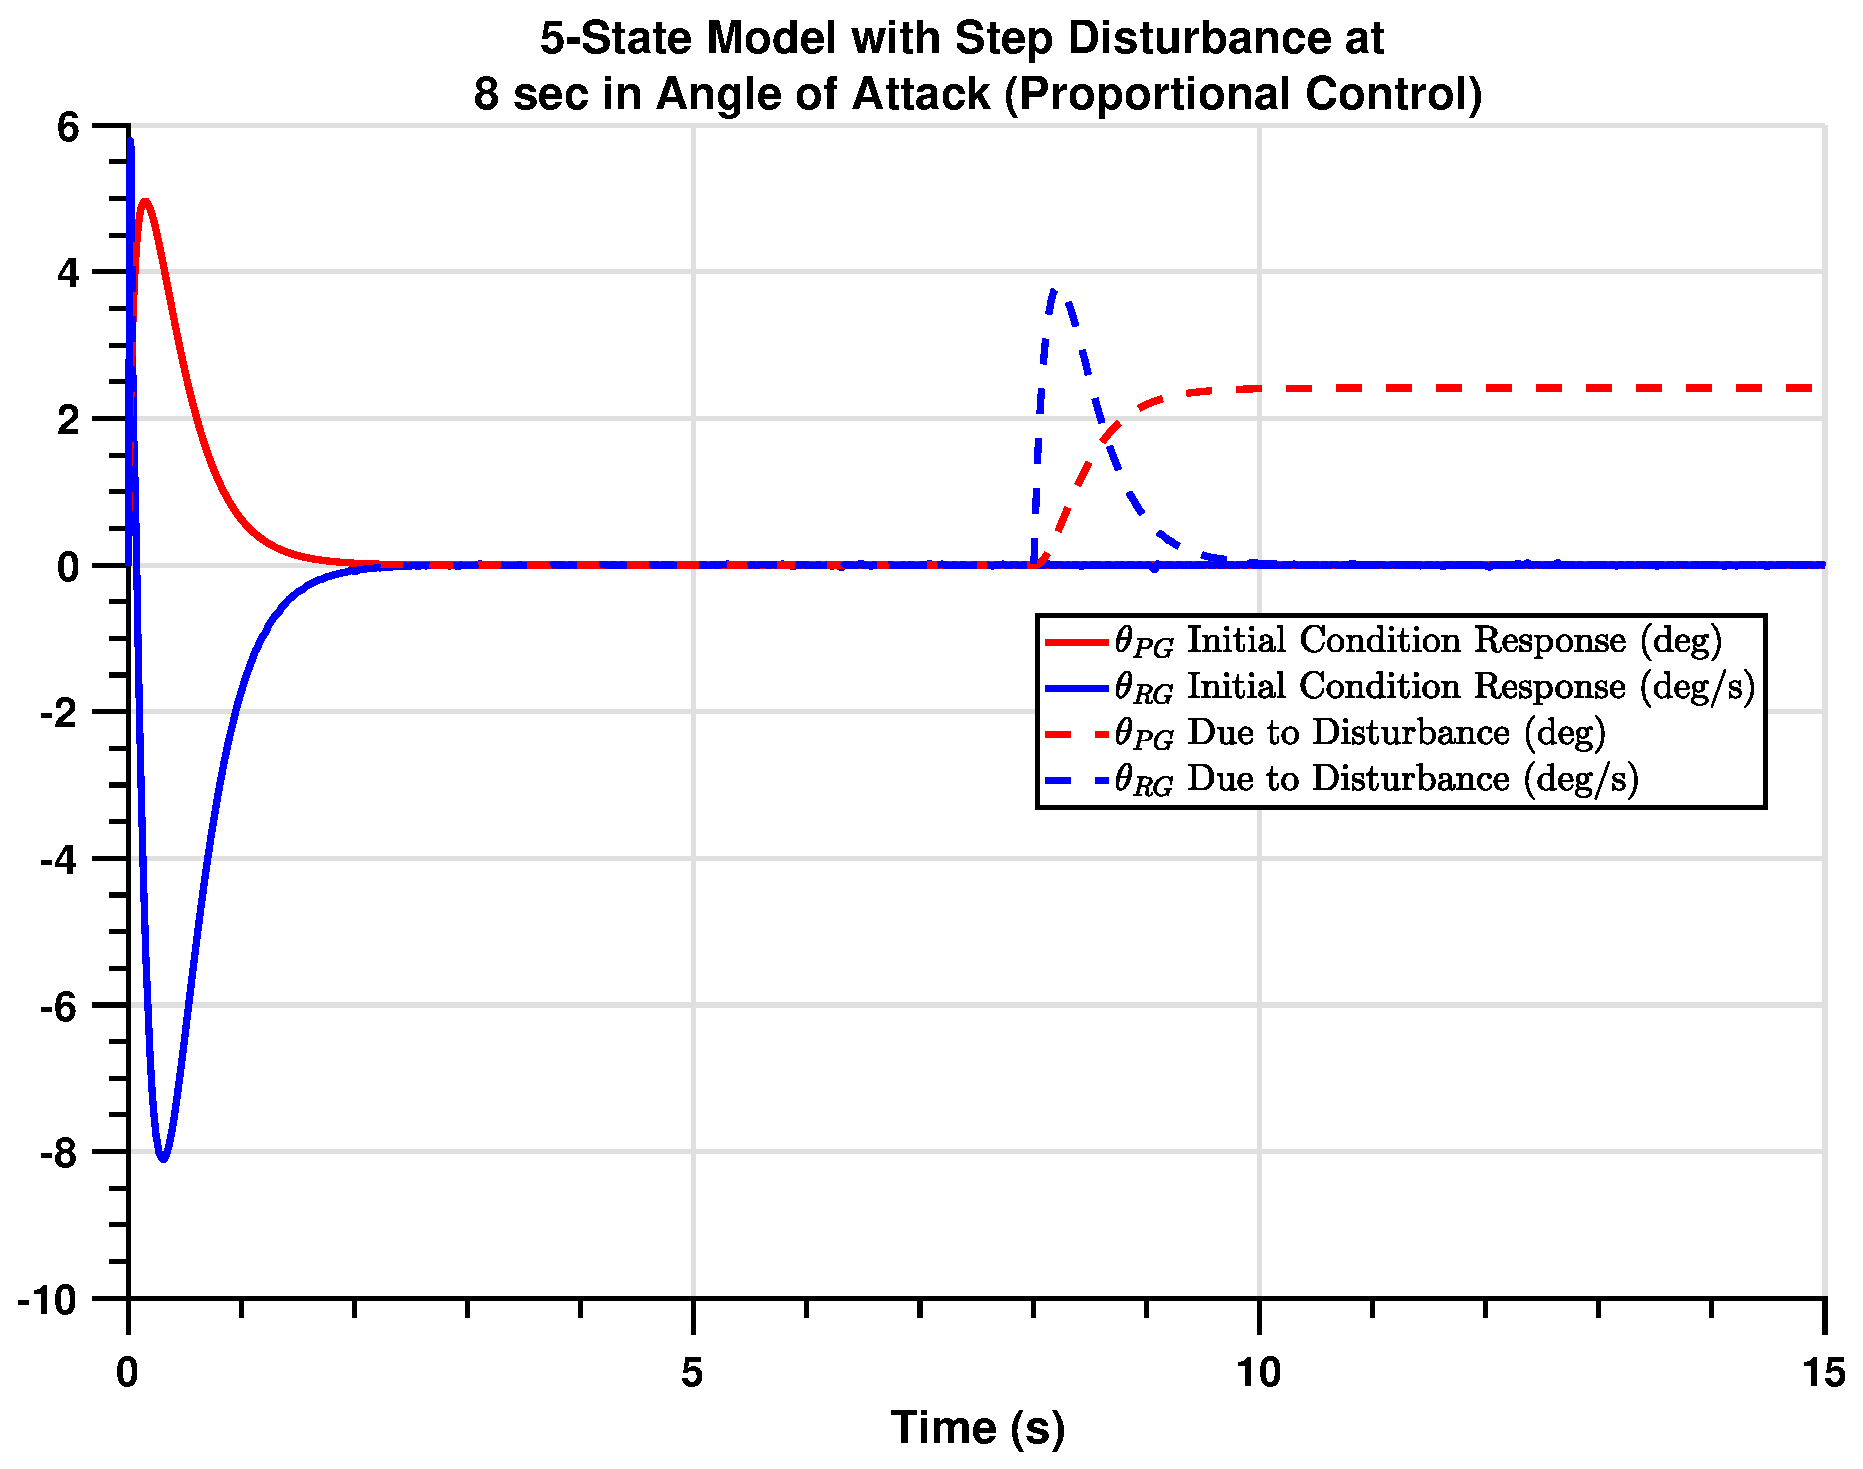
\includegraphics[width=0.8\linewidth]{disturbanceRejectionPControl}
		\caption{Proportional Control and Steady State Error Due to Step Disturbance}
		\label{fig:disturbancerejectionpcontrol}
	\end{figure}
	
	\subsubsection{Proportional and Integral Feedback Control Design}
	In order to reduce the steady state error, PI control strategy was considered next. For the two state case, this controller is translated into the following transfer function K(s) matrix. It is worth noticing that $K_P = [k_{p_1}, k_{p_2}]$ and $K_I = [k_{i_1}, 0]$ are both $1 \times 2$ vectors.
	
	\begin{equation}
	\label{eq19}
	\begin{split}
	K(s) &= 
	K_I \frac{1}{s} + K_P = \begin{bmatrix}
	k_{p_1} + \frac{k_{i_1}}{s}, & k_{p_2}
	\end{bmatrix}\\
	&=
	\left[
	\begin{array}{c | c}
	0_{2 \times 2}  & I_{2 \times 2} \\ \hline
	K_I & K_P
	\end{array}\right] \\
	\end{split}
	\end{equation}
	
	\noindent Similar to section \ref{pcontrol}, we started with the control design using MATLAB function \texttt{lqi()} to compute the gains $K_I$ and $K_P$. Later using trial and error following gains were computed for PI control.
	
	\begin{equation}
	\begin{split}
	K_P = \begin{bmatrix} -3 & -1.3 \end{bmatrix}\\
	K_I = \begin{bmatrix} -2 & 0 \end{bmatrix}\\
	\end{split}
	\end{equation}
	
	\noindent Thus, for the full 5 state model, following gain matrices can be used. 
	\begin{equation}
	\begin{split}
	K_{P_5} &= \begin{bmatrix}
	k_{p_1} & k_{p_2} \\
	0&0\\
	0&0\\
	\end{bmatrix} = \begin{bmatrix}
	-3 & -1.3\\
	0&0\\
	0&0\\
	\end{bmatrix}\\
	K_{I_5} &= \begin{bmatrix}
	k_{i_1} & k_{i_2}\\
	0&0\\
	0&0\\
	\end{bmatrix} = \begin{bmatrix}
	-2 & 0\\
	0&0\\
	0&0\\
	\end{bmatrix}
	\end{split}
	\end{equation}
	
	\noindent Full 5 state model was implemented in Simulink to simulate the closed loop response. Figure \ref{fig:model5statespiinitialcond} shows the initial condition response for PI Controller similar to first 2 states of Figure \ref{fig:disturbancerejectionpcontrol}. The limitation of Proportional feedback was steady state error to disturbance, which was evaluated in Figure \ref{fig:model5statespidisturbanceinalpha} by applying angle of attack disturbance $\alpha$ = $-5^{o}$ at 1 s. PI Controller result shows that steady state error is now maintained at zero after some transient controller effort. Similar exercise was done with the wind gust disturbance of 100 m/s (maximum possible) as shown in Figure \ref{fig:model5statespidisturbanceinwind} at 1 s. Finally, both the disturbances were applied together at different time instance to see if controller is able to recover from the applied disturbance. Overall, the designed PI controller does well in terms of performance and brings the steady state errors to 0. The primary goal of zero steady state error and stabilization of the plant is fulfilled.
	
	\begin{figure}[H]
		\centering
		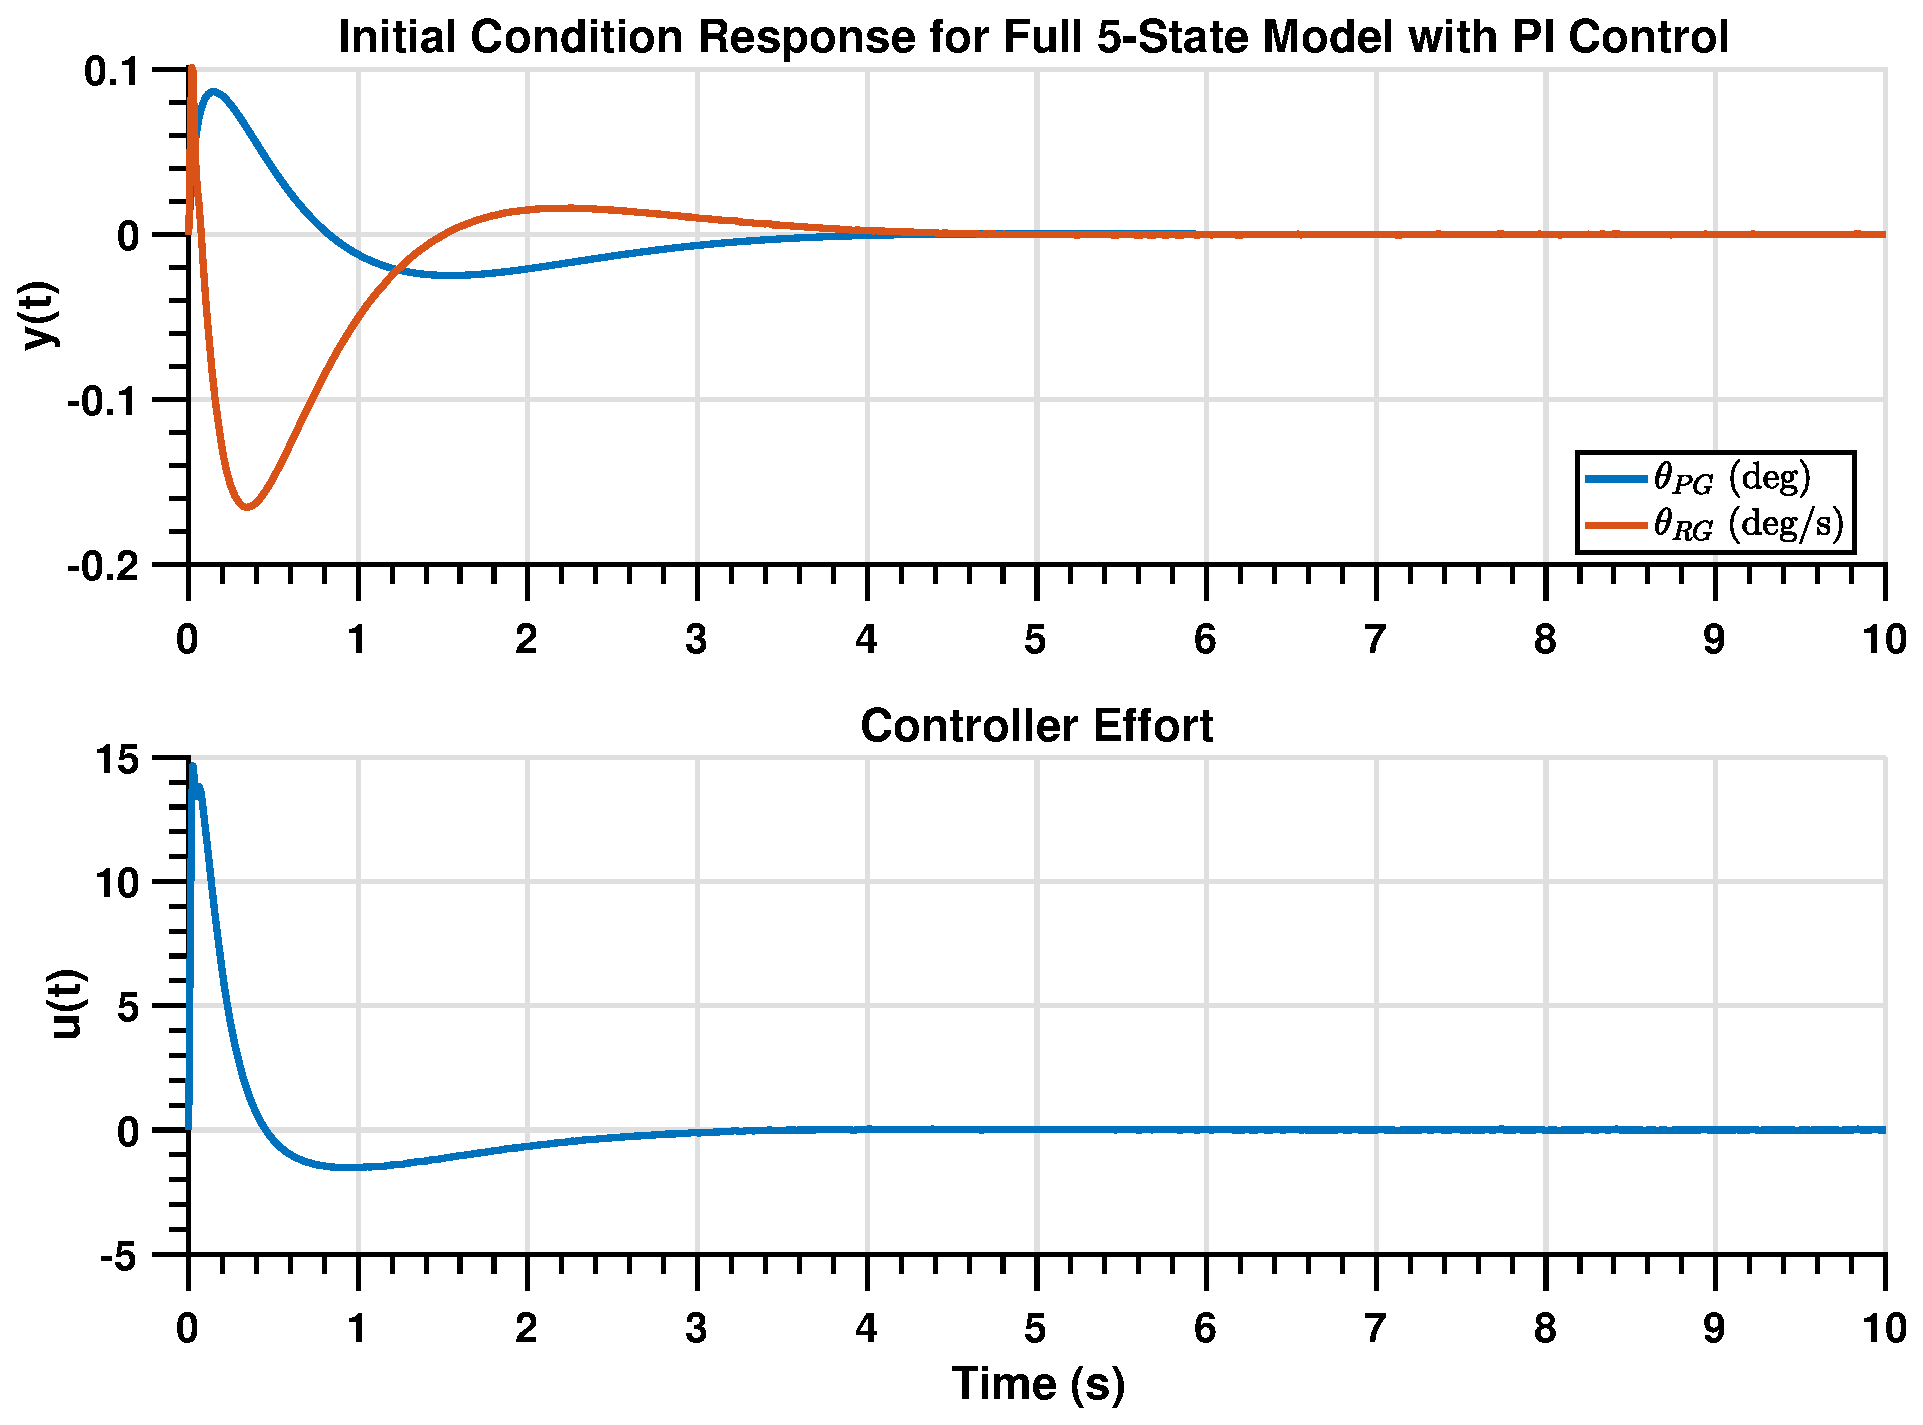
\includegraphics[width=0.8\linewidth]{LaunchVehicle_initialCond}
		\caption{Initial Condition Response with Full State PI Control}
		\label{fig:model5statespiinitialcond}
	\end{figure}
	
	\begin{figure}[H]
		\centering
		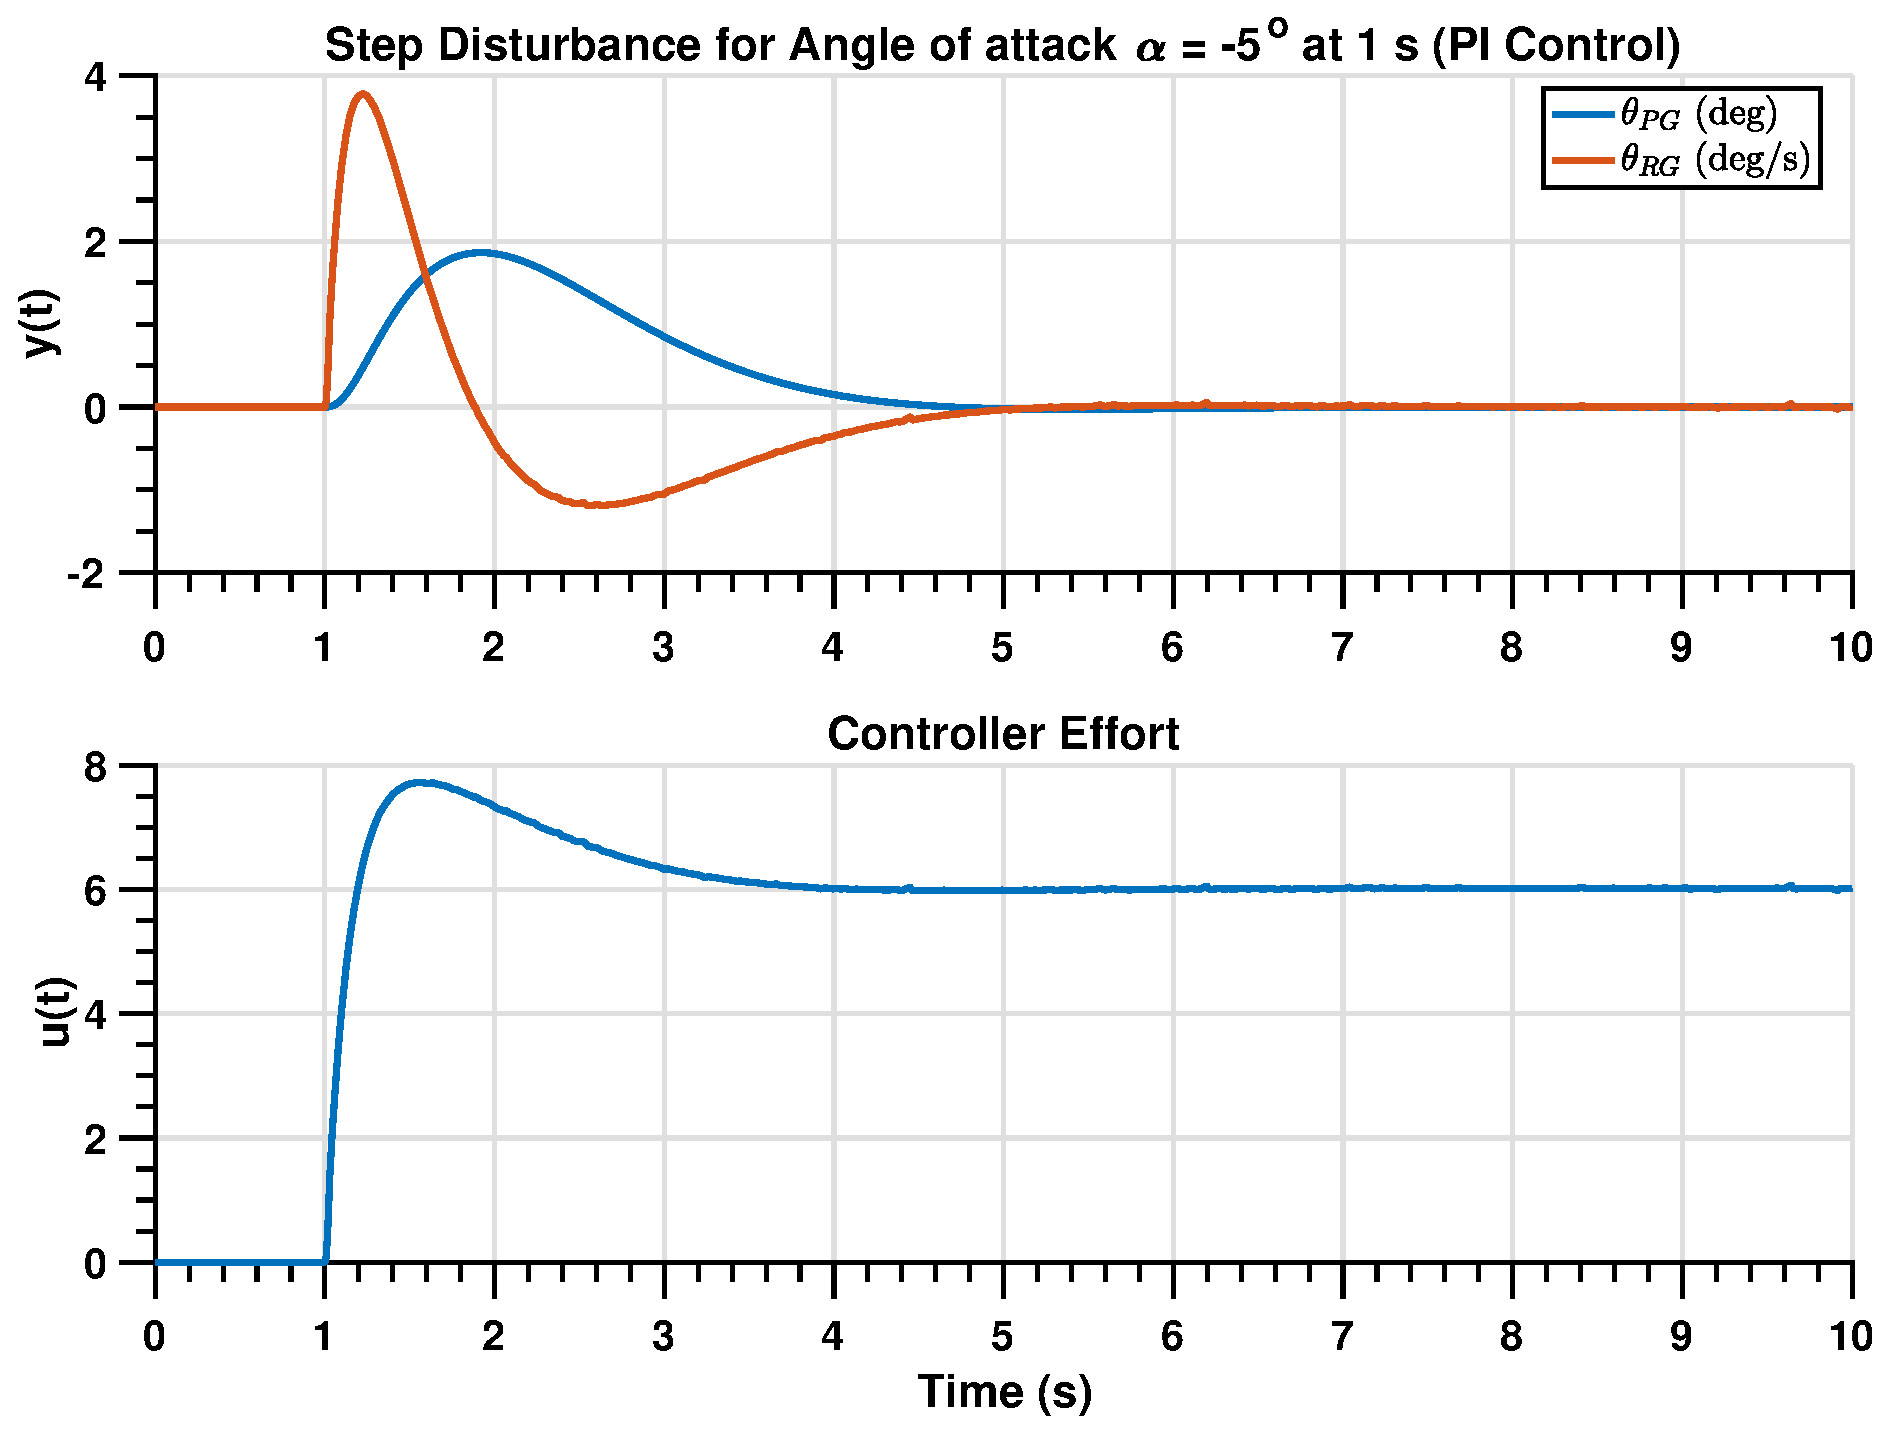
\includegraphics[width=0.8\linewidth]{LaunchVehicle_DisturbanceInAlpha}
		\caption{Step Disturbance for $\alpha$ = $-5^{o}$ at 1 s}
		\label{fig:model5statespidisturbanceinalpha}
	\end{figure}
	
	\begin{figure}[H]
		\centering
		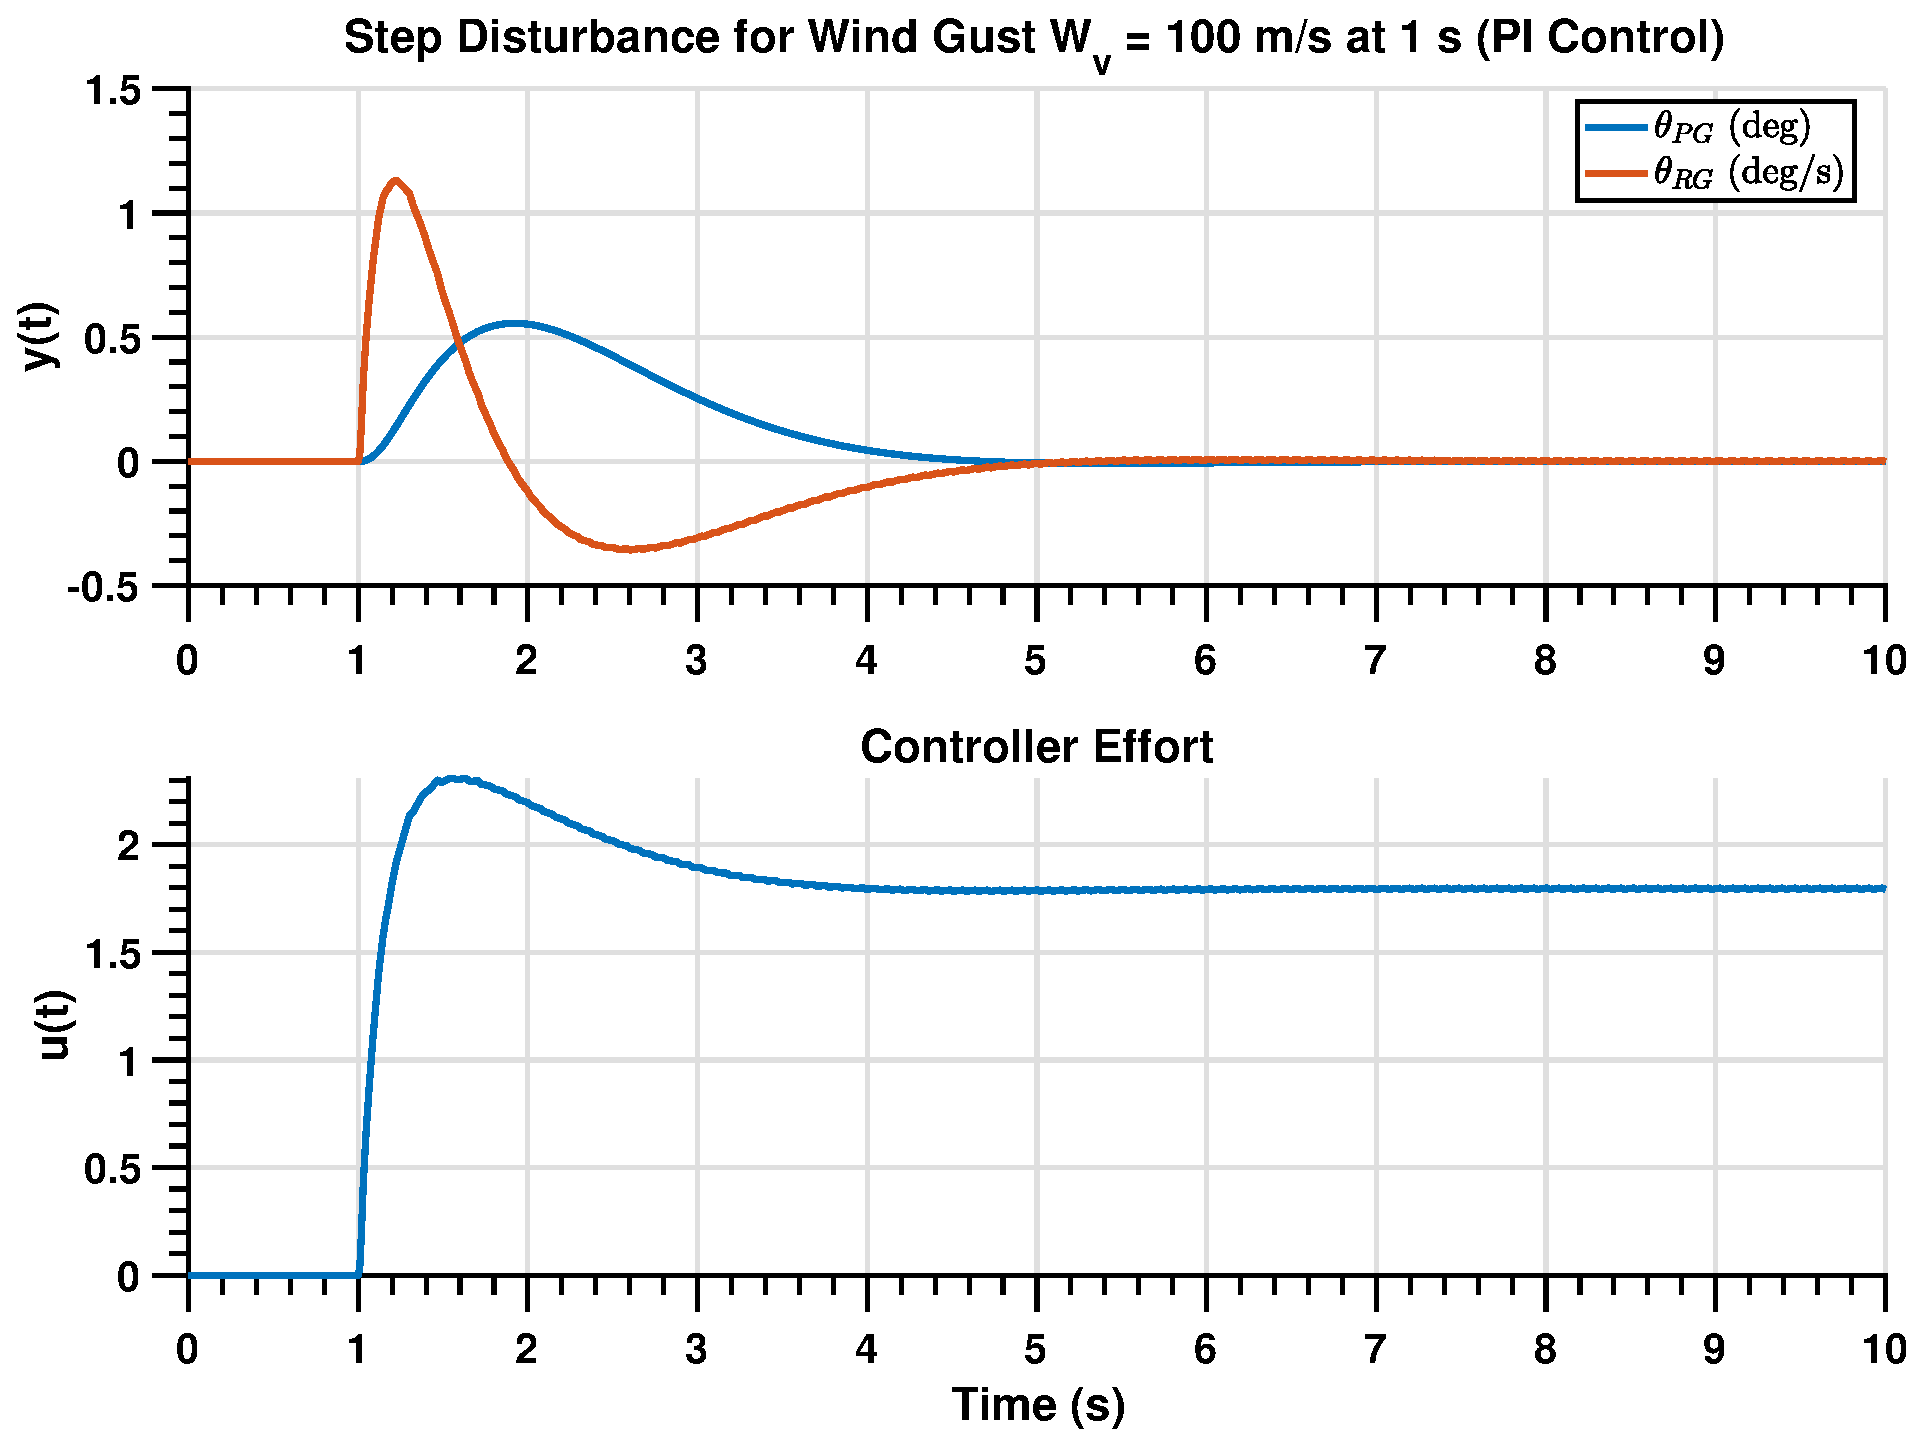
\includegraphics[width=0.8\linewidth]{LaunchVehicle_DisturbanceInWind}
		\caption{Step Disturbance as Wind Gust $W_v$ = 100 m/s at 1 s}
		\label{fig:model5statespidisturbanceinwind}
	\end{figure}
	
	\subsection{Nominal Closed Loop Analysis}
	\subsubsection{Poles of Controller K(s)}
	For Proportional and Integral controller, the poles are located at the origin as can be seen from equation \ref{eq19}.
	
	\subsubsection{Closed Loop Poles, Damping and Natural Frequency}
	Compared to open loop poles, it is verified that feedback stabilized the system since all the poles are having negative real part. Following table shows individual pole and damping characteristics. It can be observed that the unstable pole is now transformed in to stable complex conjugate pair of poles with damping ratio of 0.8, which is well damped. \texttt{linmod()} function was used to linearize the Simulink model and get state space matrices for closed loop. Further the closed loop poles or eigenvalues were verified from previous calculation.
	
	\begin{center}
		\begin{tabular}{ |p{2.4cm}|p{2.3cm}|p{2cm}|p{3.5cm}||p{3.5cm}|  }
			\hline
			\multicolumn{5}{|c|}{Summary of Closed Loop Poles} \\
			\hline
			Poles ($\underline{\lambda}$)  & Damping ($\zeta$) & Frequency (rad/s) & Time Constant (s) & Behavior\\ \hline
			-52.9 + 131$j$ & 0.373 & 142 & 0.0189 & Fast\\
			-52.9 - 131$j$  & 0.373 & 142 & 0.0189 & Fast\\
			-1.21  + 0.93$j$ & 0.8 & 1.51 & 0.829 & Well-Damped\\
			-1.21  - 0.93$j$ & 0.8 & 1.51 & 0.829 & Well-Damped\\
			-6.88 & 1 & 6.88 & 0.145 & Stable\\
			-26.5 & 1 & 26.5 & 0.0378 & Non-Dominant\\
			\hline
		\end{tabular}
	\end{center}
	
	\subsubsection{Frequency Response}
	For 2 states model, the Input loop transfer function is given by,
	
	\begin{equation}
	L_{I_2} = KG =
	\left[
	\begin{array}{c | c}
	A_{Li_2} & B_{Li_2}\\ \hline
	C_{Li_2} & D_{Li_2}
	\end{array}\right] \\
	\end{equation}
	Where, using cascade state-space manipulations,
	\begin{equation}
	\begin{split}
	A_{Li_2}  = \begin{bmatrix}
	0_{2 \times 2} & I_2\\
	0_{2 \times 2} & A_2\\
	\end{bmatrix},
	B_{Li_2}  =  \begin{bmatrix} 
	0_{2 \times 1} & B_2 \\
	\end{bmatrix},
	C_{Li_2}  = \begin{bmatrix} 
	K_{I} & K_{P} \\
	\end{bmatrix},
	D_{Li_2}  = 0
	\end{split}
	\end{equation}
	
	\noindent Plotting above input loop transfer function, gain cross over frequency was found to be 9.88 rad/sec. It is desired for robust stability for unstable low pass type system that gain crossover frequency $W_c > 2*a$, where $a$ is unstable open loop pole. In this case, it is 1.99 $\implies W_c > 4$ criteria is satisfied as shown in the Figure \ref{fig:bode2states}.
	
	\begin{figure}[H]
		\centering
		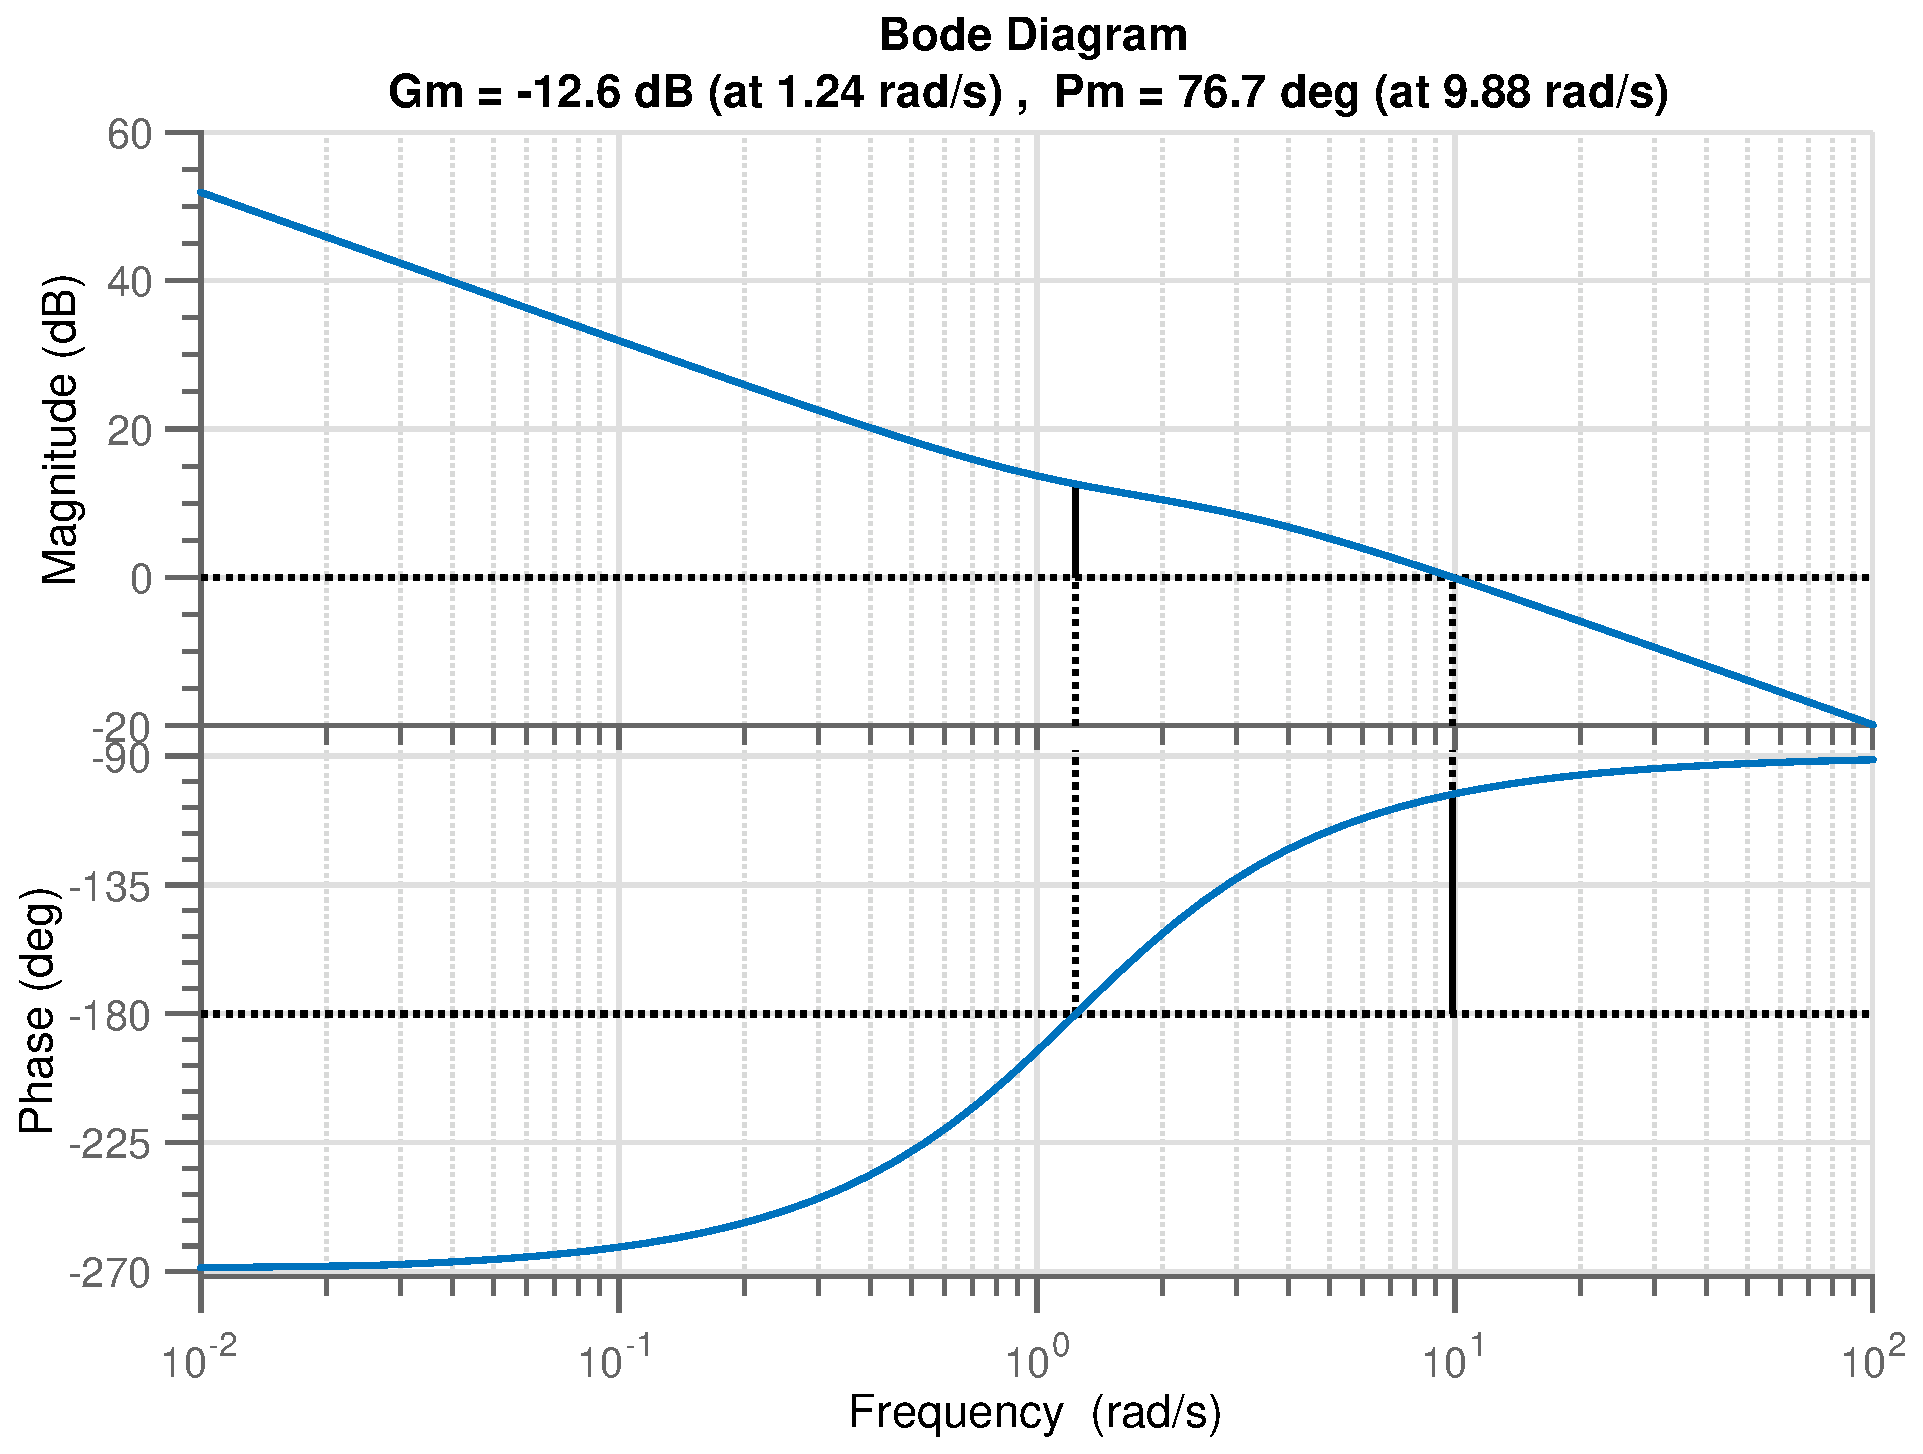
\includegraphics[width=0.75\linewidth]{InputLoopBode_2states}
		\caption{Bode Plot of Input Loop Transfer Function (2-State Model)}
		\label{fig:bode2states}
	\end{figure}
	
	\begin{figure}[H]
		\centering
		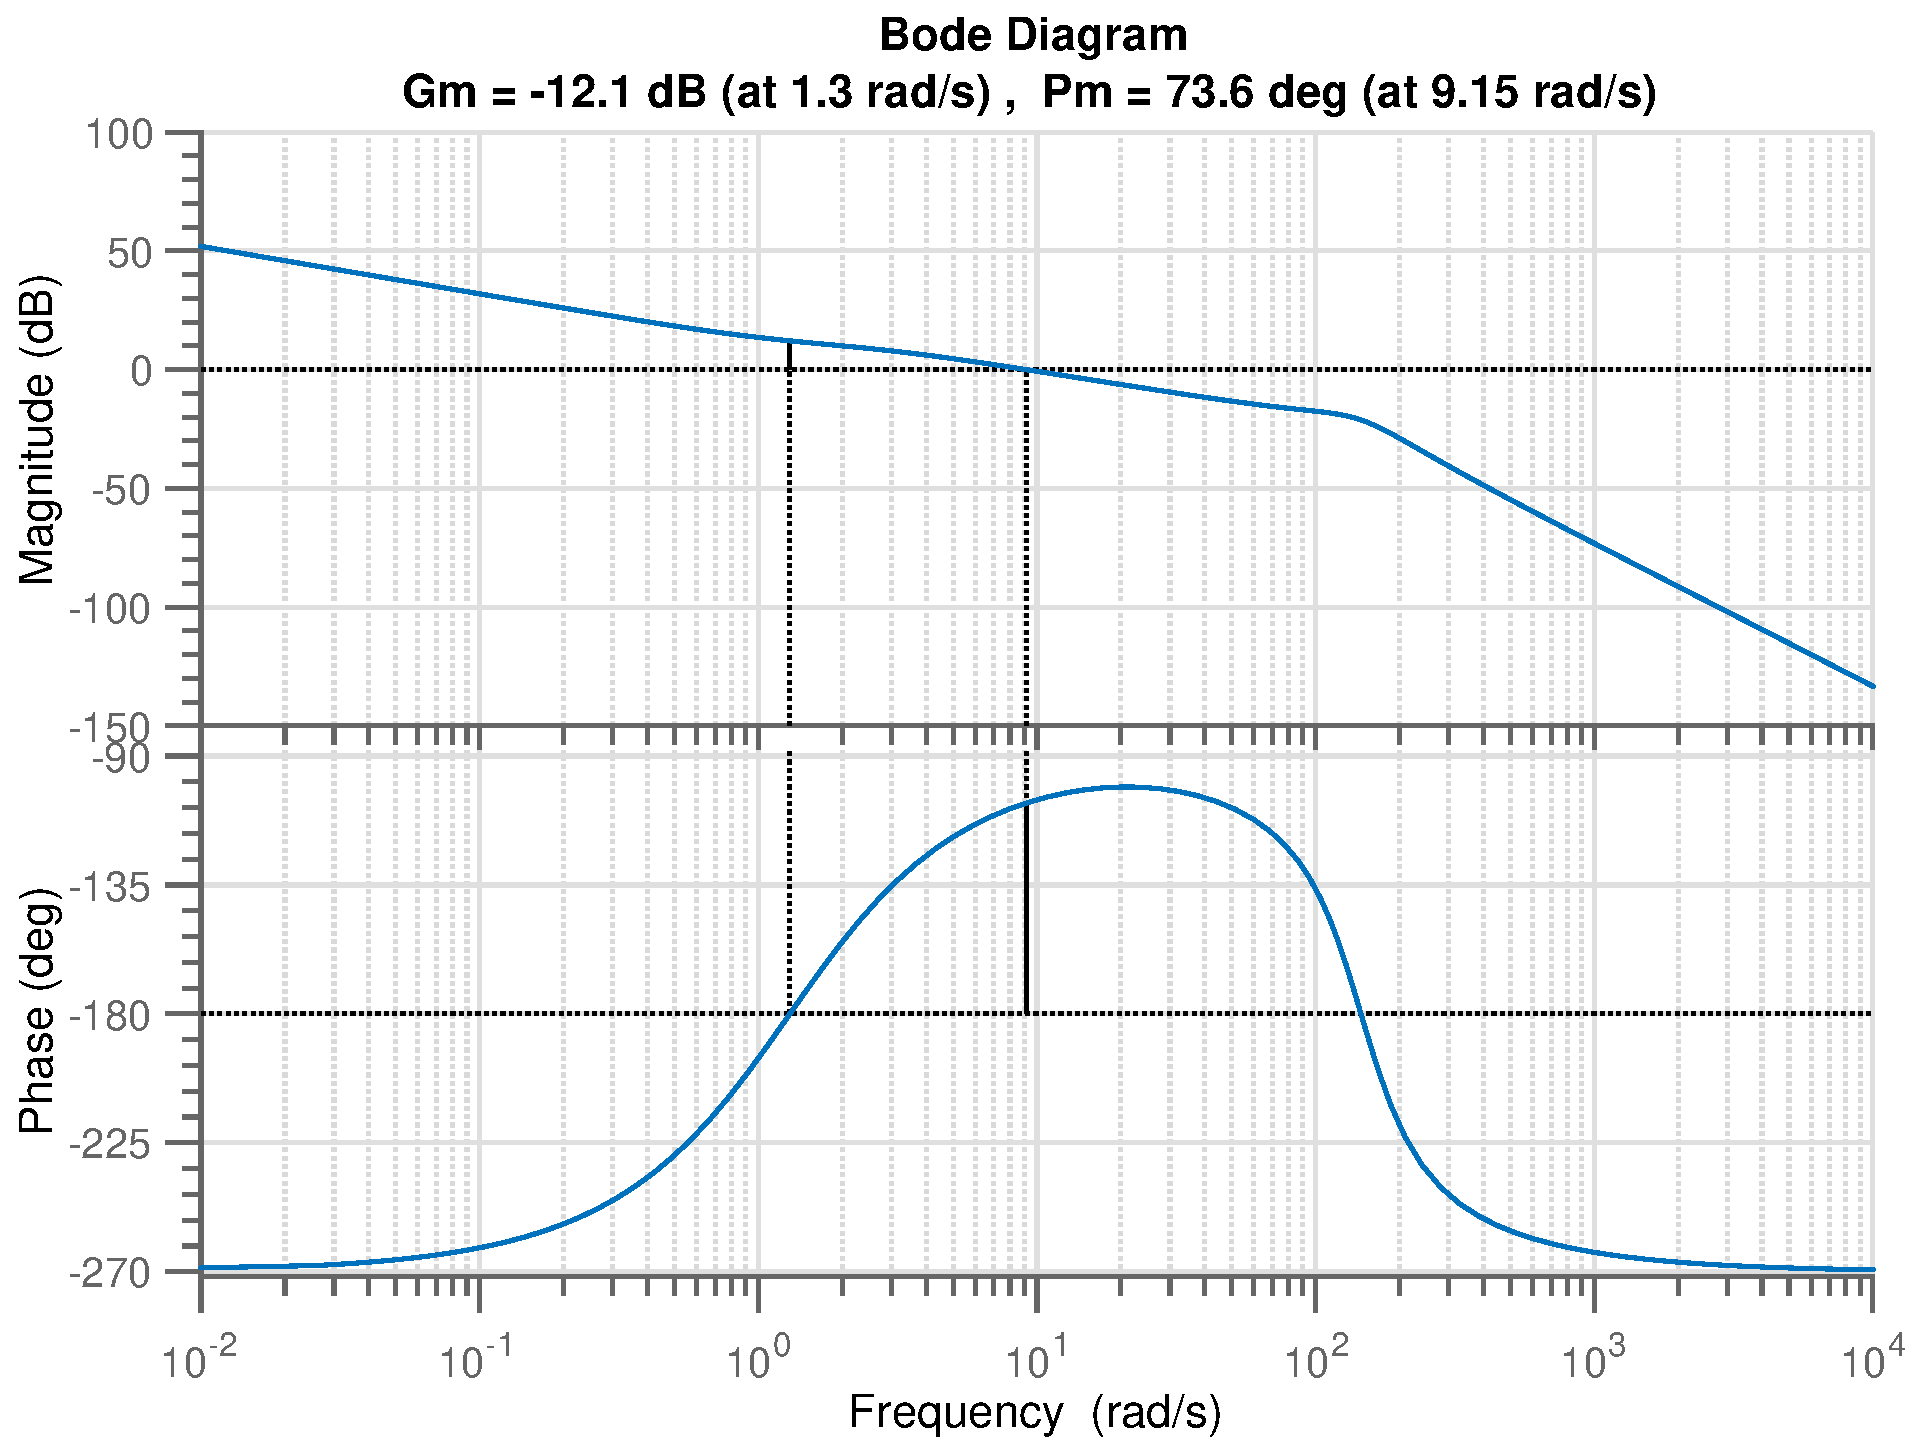
\includegraphics[width=0.75\linewidth]{bode_5states1}
		\caption{Bode Plot of Input Loop Transfer Function (5-State Model)}
		\label{fig:bode_5states1}
	\end{figure}
	
	\subsubsection{Time Domain Performance}
	Step Response was plotted in Simulink for $5^{o}$ of reference tracking as shown in the Figure \ref{fig:model5statespistepresponse}. It can be seen that steady state error in tracking performance is 0. The response characteristics were computed using MATLAB command \texttt{stepinfo(y,t)} and are summarized in the following table. 
	
	\begin{figure}[H]
		\centering
		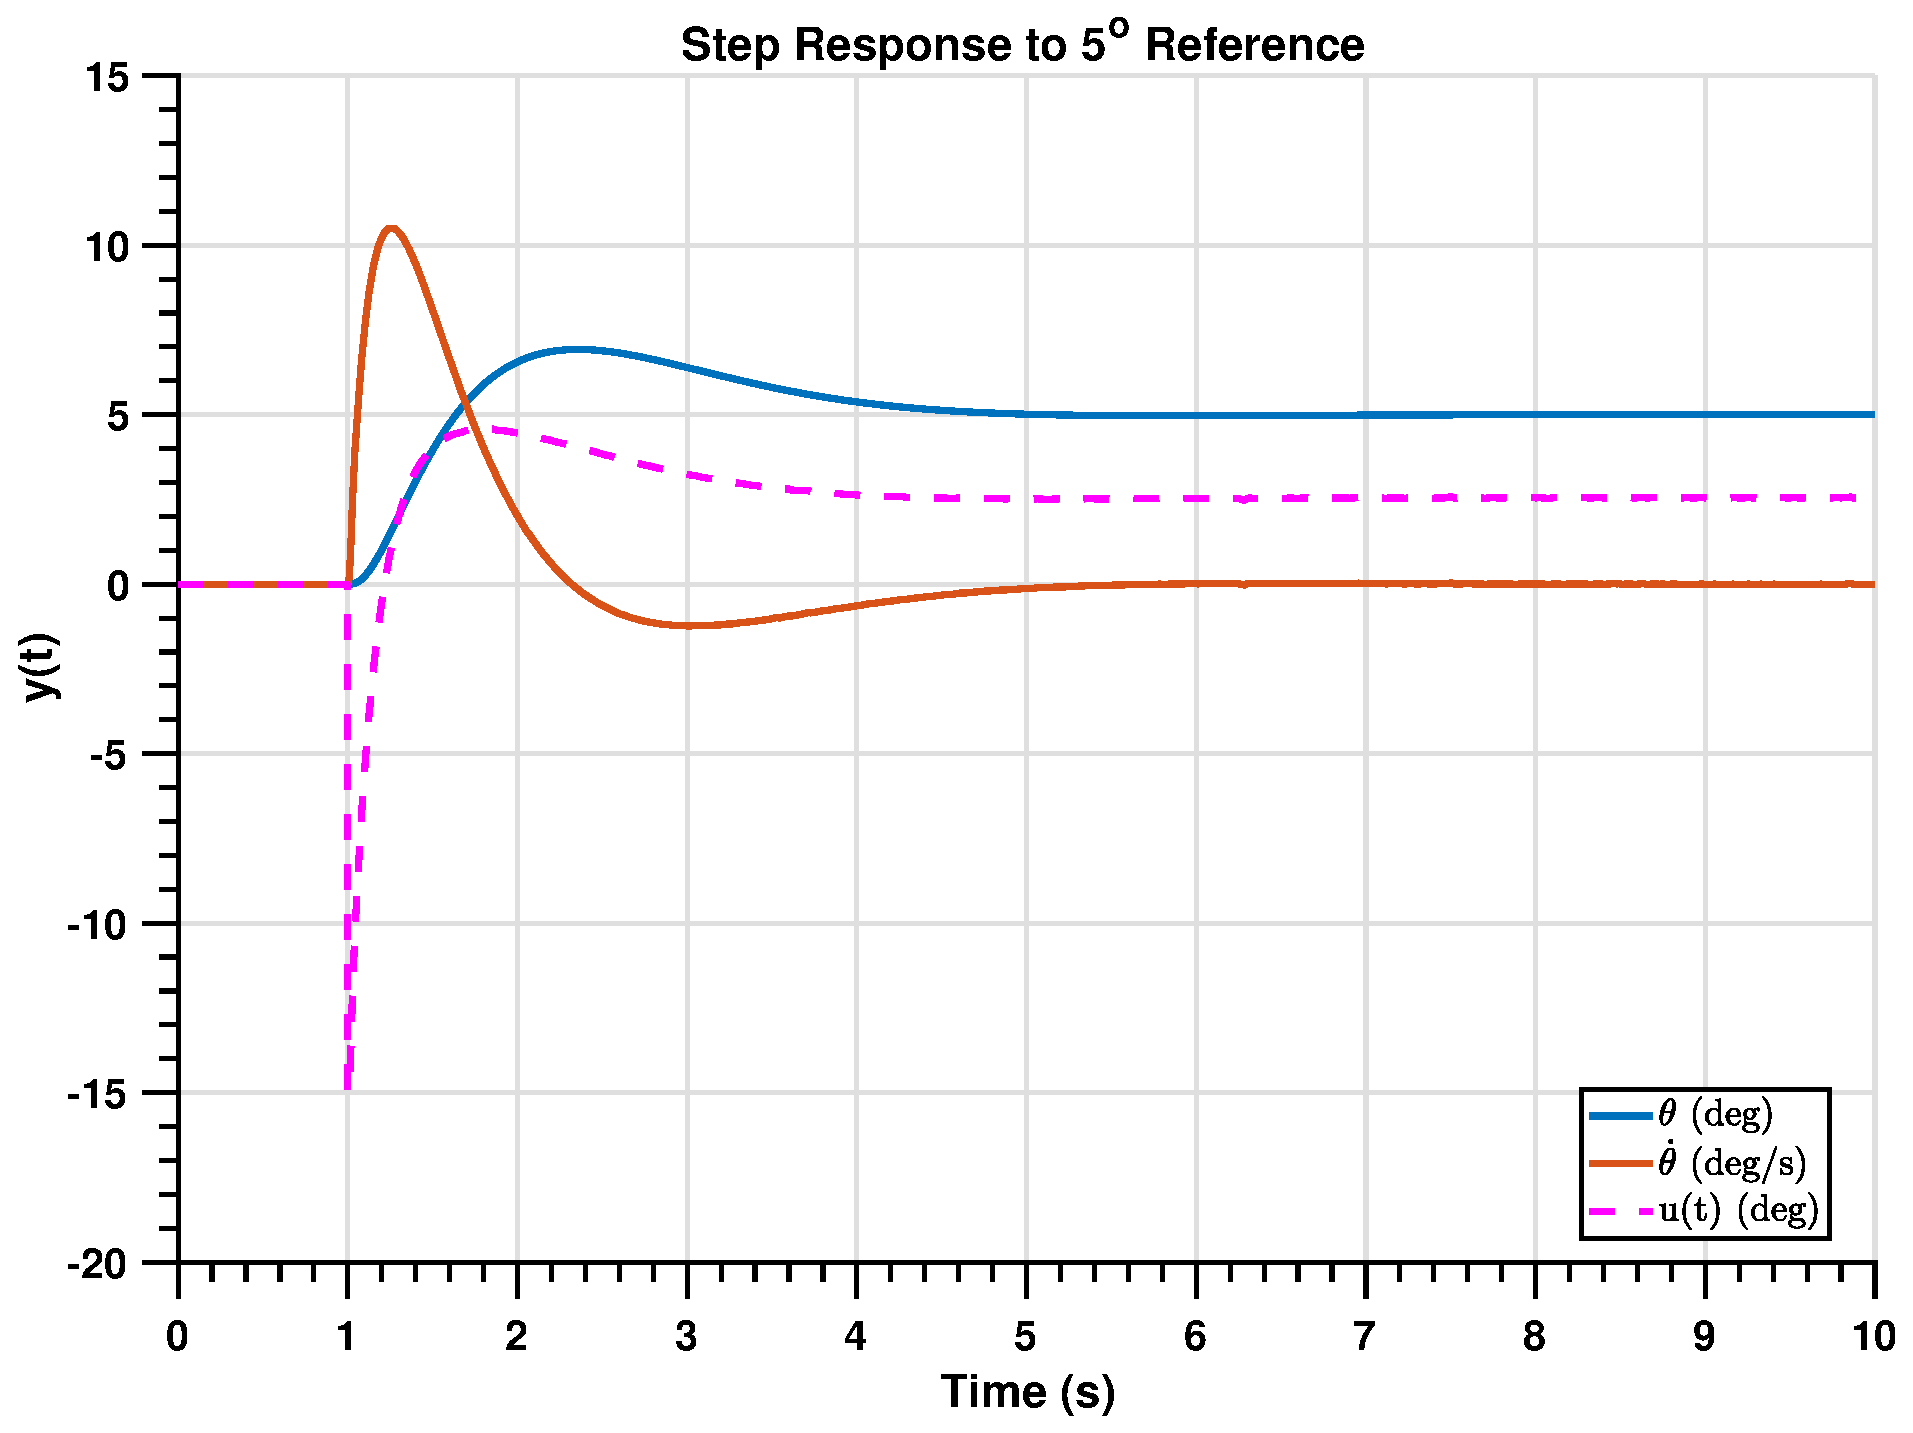
\includegraphics[width=0.8\linewidth]{LaunchVehicle_StepResponse}
		\caption{Step Response of Closed Loop System (5-State Model)}
		\label{fig:model5statespistepresponse}
	\end{figure}
	\begin{center}
		\begin{tabular}{ |p{4cm}|p{2.4cm}| }
			\hline
			\multicolumn{2}{|c|}{Step Response Statistics} \\
			\hline
			Rise time ($s$)& 0.42797 \\
			Settling Time ($s$)& 4.5917 \\
			Settling Min ($s$)& 4.5134\\
			Settling Max ($s$)& 6.9247\\
			Overshoot ($\%$) & 38.48 \\
			Undershoot ($\%$) & 0\\
			Peak & 6.9247\\
			Peak Time ($s$)& 2.3465\\
			\hline
		\end{tabular}
	\end{center}
	\noindent It is evident that the chosen control strategy provided desired design specifications, such as settling time less than 5 s, rise time less then 2 s. A compromise was made to accept more overshoot ($\approx$ 38$\%$) in return for faster rise time for step reference tracking. Actuator effort was observed to be reasonable which was maximum of $15^{o}$.
	
	\subsubsection{Nominal Performance}
	For Nominal Performance, sensitivity $S(j\omega)$ plot is shown in the Figure \ref{fig:sigmafreqplotfors11}.  Designed bandwidth frequency was chosen to be $\omega_b^*$ = 1.05 rad/s. Based on the steady state error requirement $A$ was selected to be 0.1 and to suppress or account for the high frequency neglected dynamics $M$ was chosen to be 2. Following guidelines from page 62 of \cite{cite3}, weights for the sensitivity transfer function then becomes, 
	
	\begin{equation}
	W_p = \frac{s/M + \omega_b^*}{s + \omega_b^*A} = \frac{0.5 s +1.05 }{s + 0.105}
	\end{equation} 
	
	\noindent Nominal performance test is given by,
	\begin{equation}
	\norm{W_P S}_{\infty} < 1
	\end{equation}
	
	\noindent Sensitivity and weighted sensitivity transfer functions are plotted in the Figure \ref{fig:sigmafreqplotfors11}. It is evident that singular values (i.e. magnitude for SISO transfer function) of the weighted sensitivity stays below 1 or 0 dB. That satisfies nominal performance criteria as discussed in \cite{cite3}.
	
	\begin{figure}[H]
		\centering
		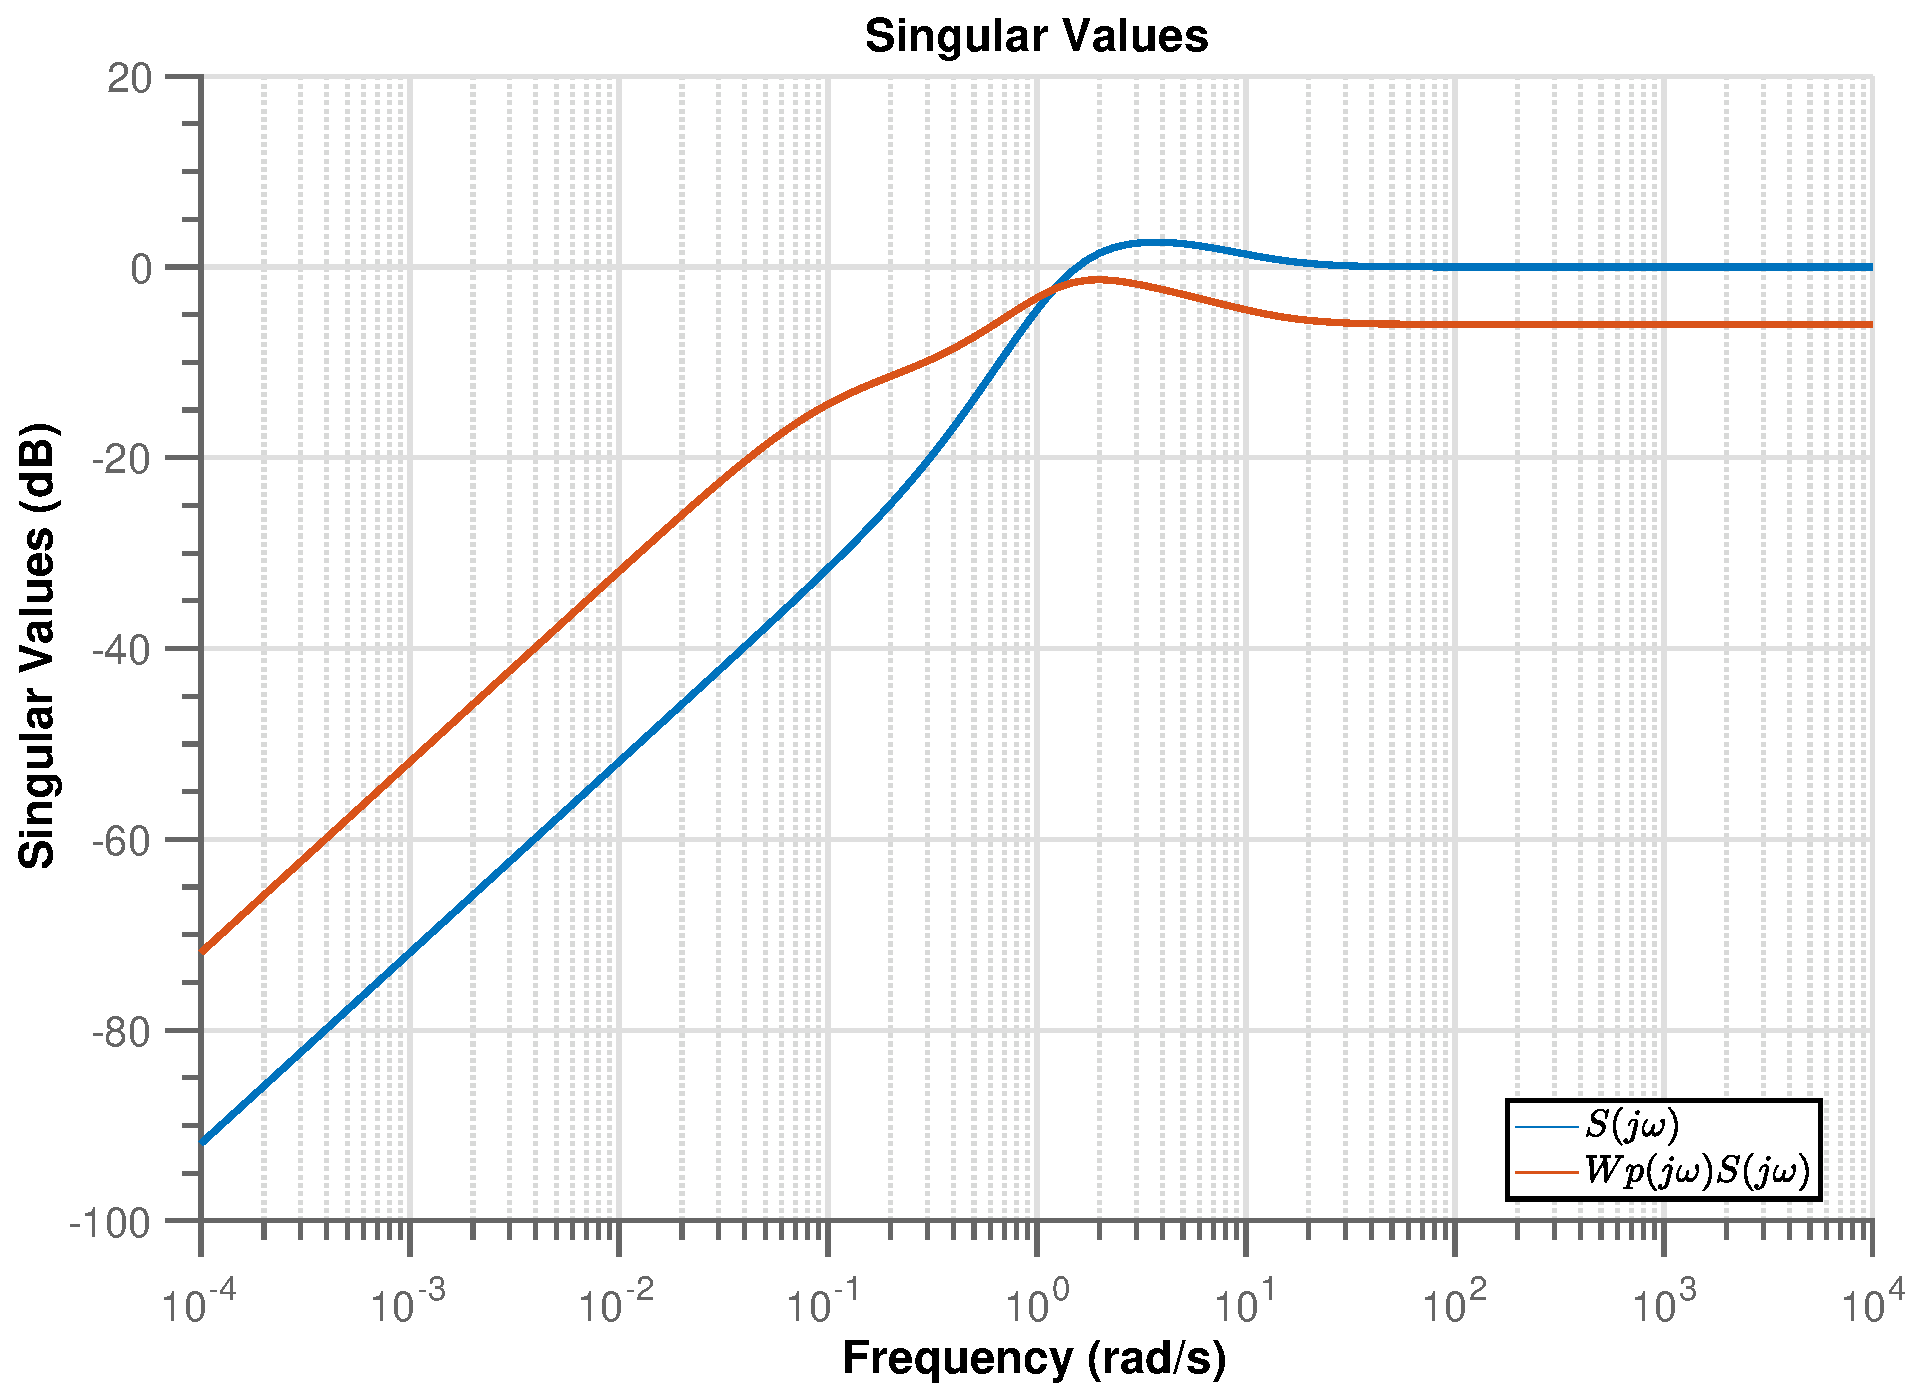
\includegraphics[width=0.8\linewidth]{sigmaFreqPlotForS11}
		\caption{Singular Values as function of frequency}
		\label{fig:sigmafreqplotfors11}
	\end{figure}
	
	\subsubsection{Robust Stability}
	Robust Stability describes a system being stable in the presence of uncertainties. Based on the \cite{cite3} it can be verified by checking the following test. 
	
	\begin{equation}
	\norm{W_I T_I}_{\infty} < 1
	\end{equation}
	
	\noindent Using \texttt{linmod} command in MATLAB, Simulink model was linearized to find the complementary sensitivity transfer function $T_I$. $W_I$ was chosen as following,
	
	\begin{equation}
	W_I = \frac{\tau s + r_{0}}{(\tau/r_{\infty})s + 1}
	\end{equation} 
	
	\noindent Where, $r_{0}$ is relative uncertainty at steady-state, $1/\tau$ is the approximate frequency at which the relative uncertainty reaches 100\%, $r_{\infty}$ is the magnitude of the weight at high frequency. Based on the provided guidelines in \cite{cite3}, we choose, $\tau$ = 1/25, $r_{0}$ = 0.05, $r_{\infty}$ = 2. Thus the weighting transfer function becomes,  
	
	\begin{equation}
	W_I = \frac{(1/25) s + 0.05}{(1/24)s + 1}
	\end{equation} 
	
	\noindent Launch vehicle elastic mode gets excited at higher frequency than 25 rad/sec, thus it can be assumed to be 100\% uncertainty above that frequency. Singular value plot for $W_I T_I$ is shown in the Figure below. The relative uncertainty at steady state is approximately 5\% (-26 dB) and high frequency magnitude is acceptable with the factor of 2 (compromise at higher frequency).
	
	\begin{figure}[H]
		\centering
		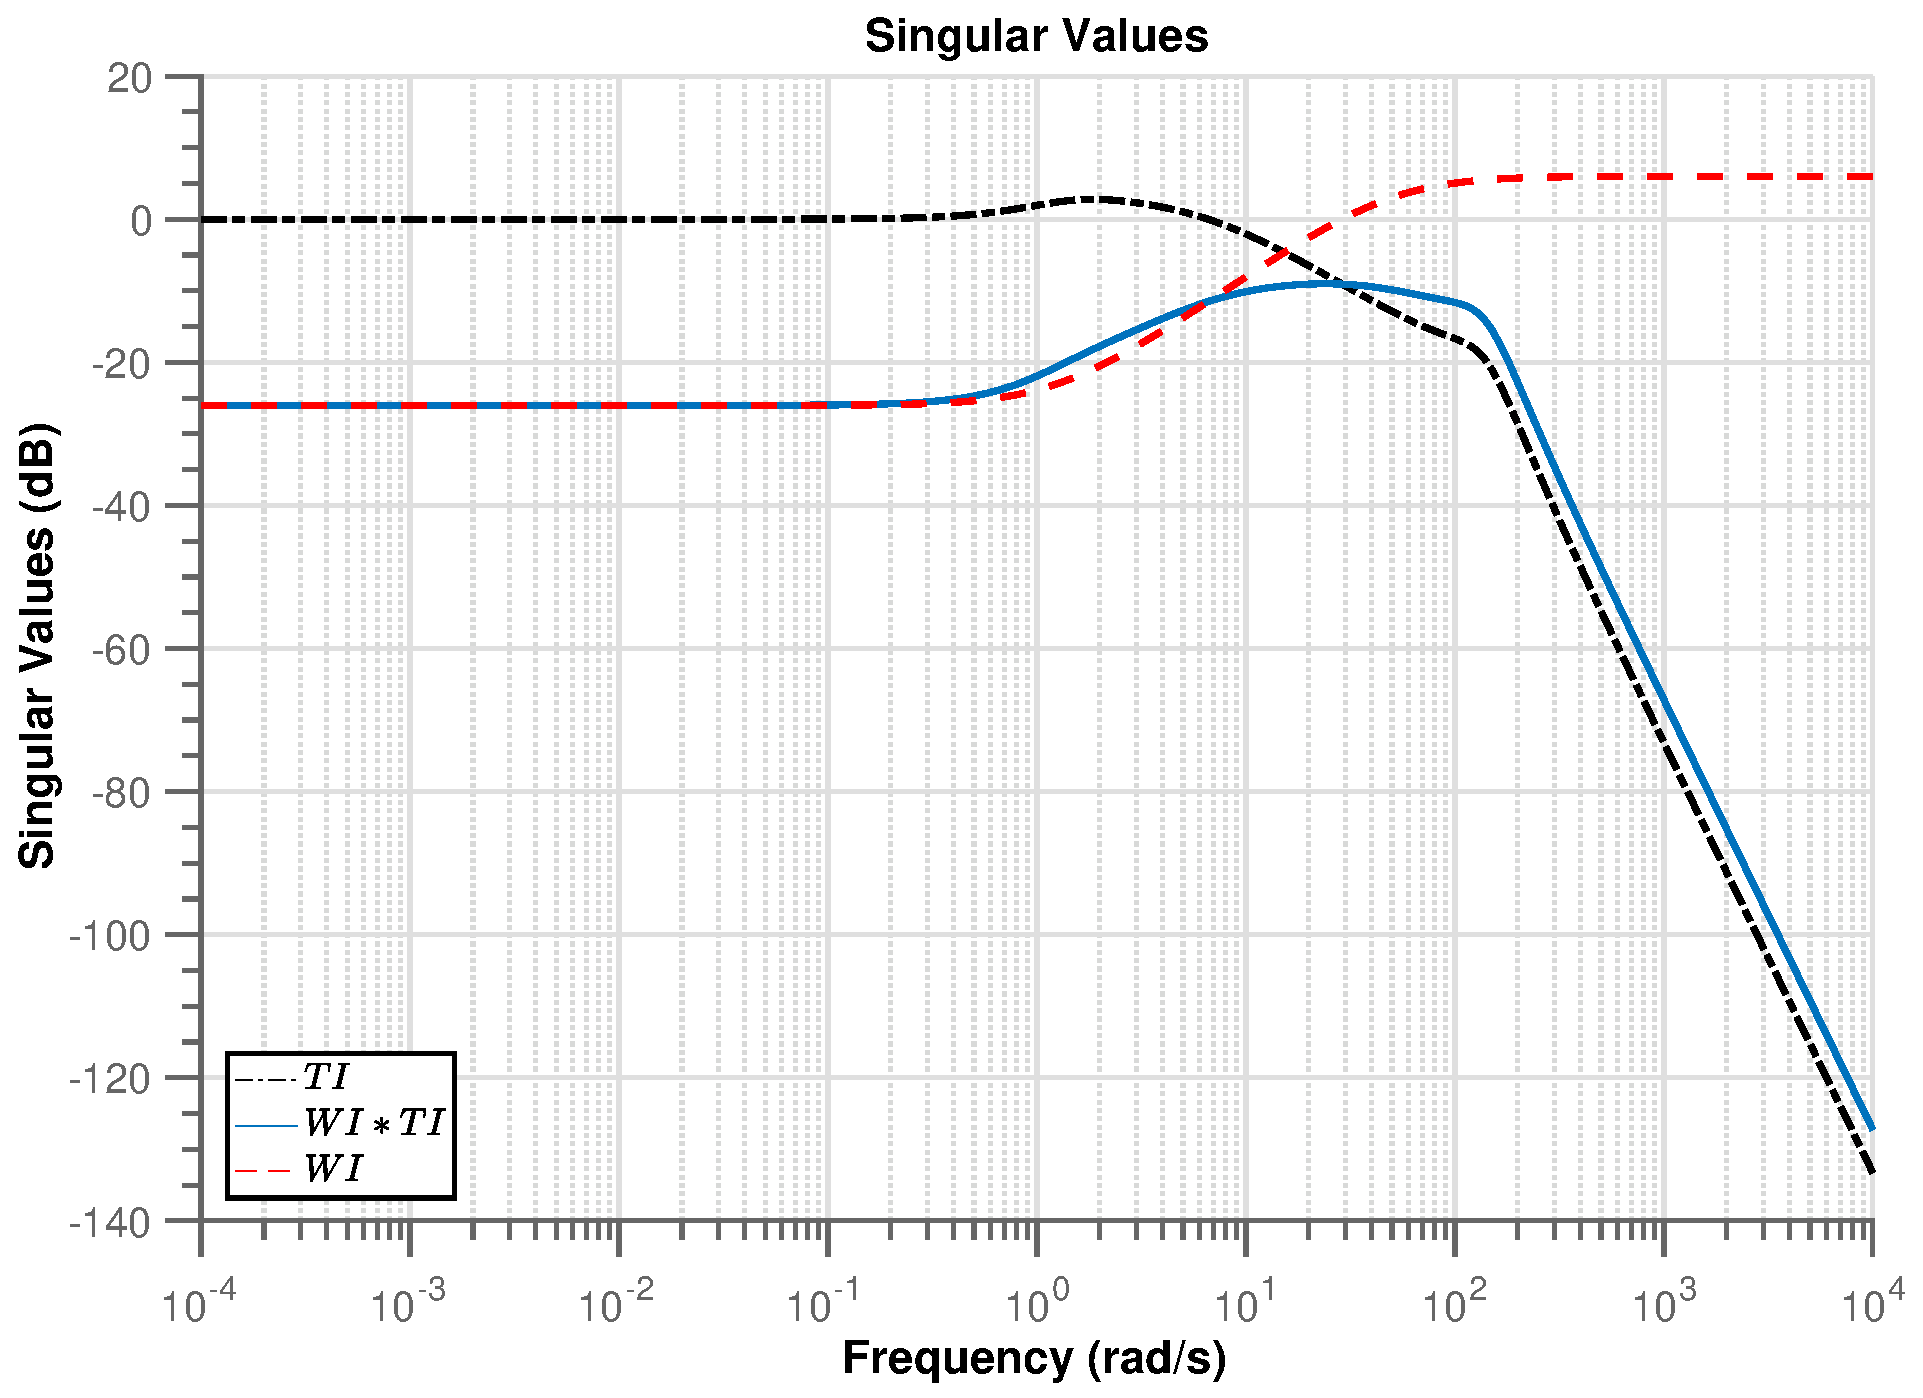
\includegraphics[width=0.8\linewidth]{SigmaOfWiTi}
		\caption{Singular Value Plot for WI*TI}
		\label{fig:sigmaofwiti}
	\end{figure}
	
	\noindent It can be seen from Figure \ref{fig:sigmaofwiti} that the $H_{\infty}$ norm of $W_I T_I$ is less than 1, thus satisfying the Robust Stability test. The peak value for $W_{I}$ is 6.02 dB. Using the provided RS analysis script, structured singular value upper bounds for 2 Sensors and 1 Actuator were computed for multiplicative perturbation which are shown in the Figure \ref{fig:SSVUpperBNDS}. Typically, the picking behavior as shown in this plot is expected. Following section describes the block diagonal uncertainty that was considered in this analysis.
	
	\begin{figure}[H]
		\centering
		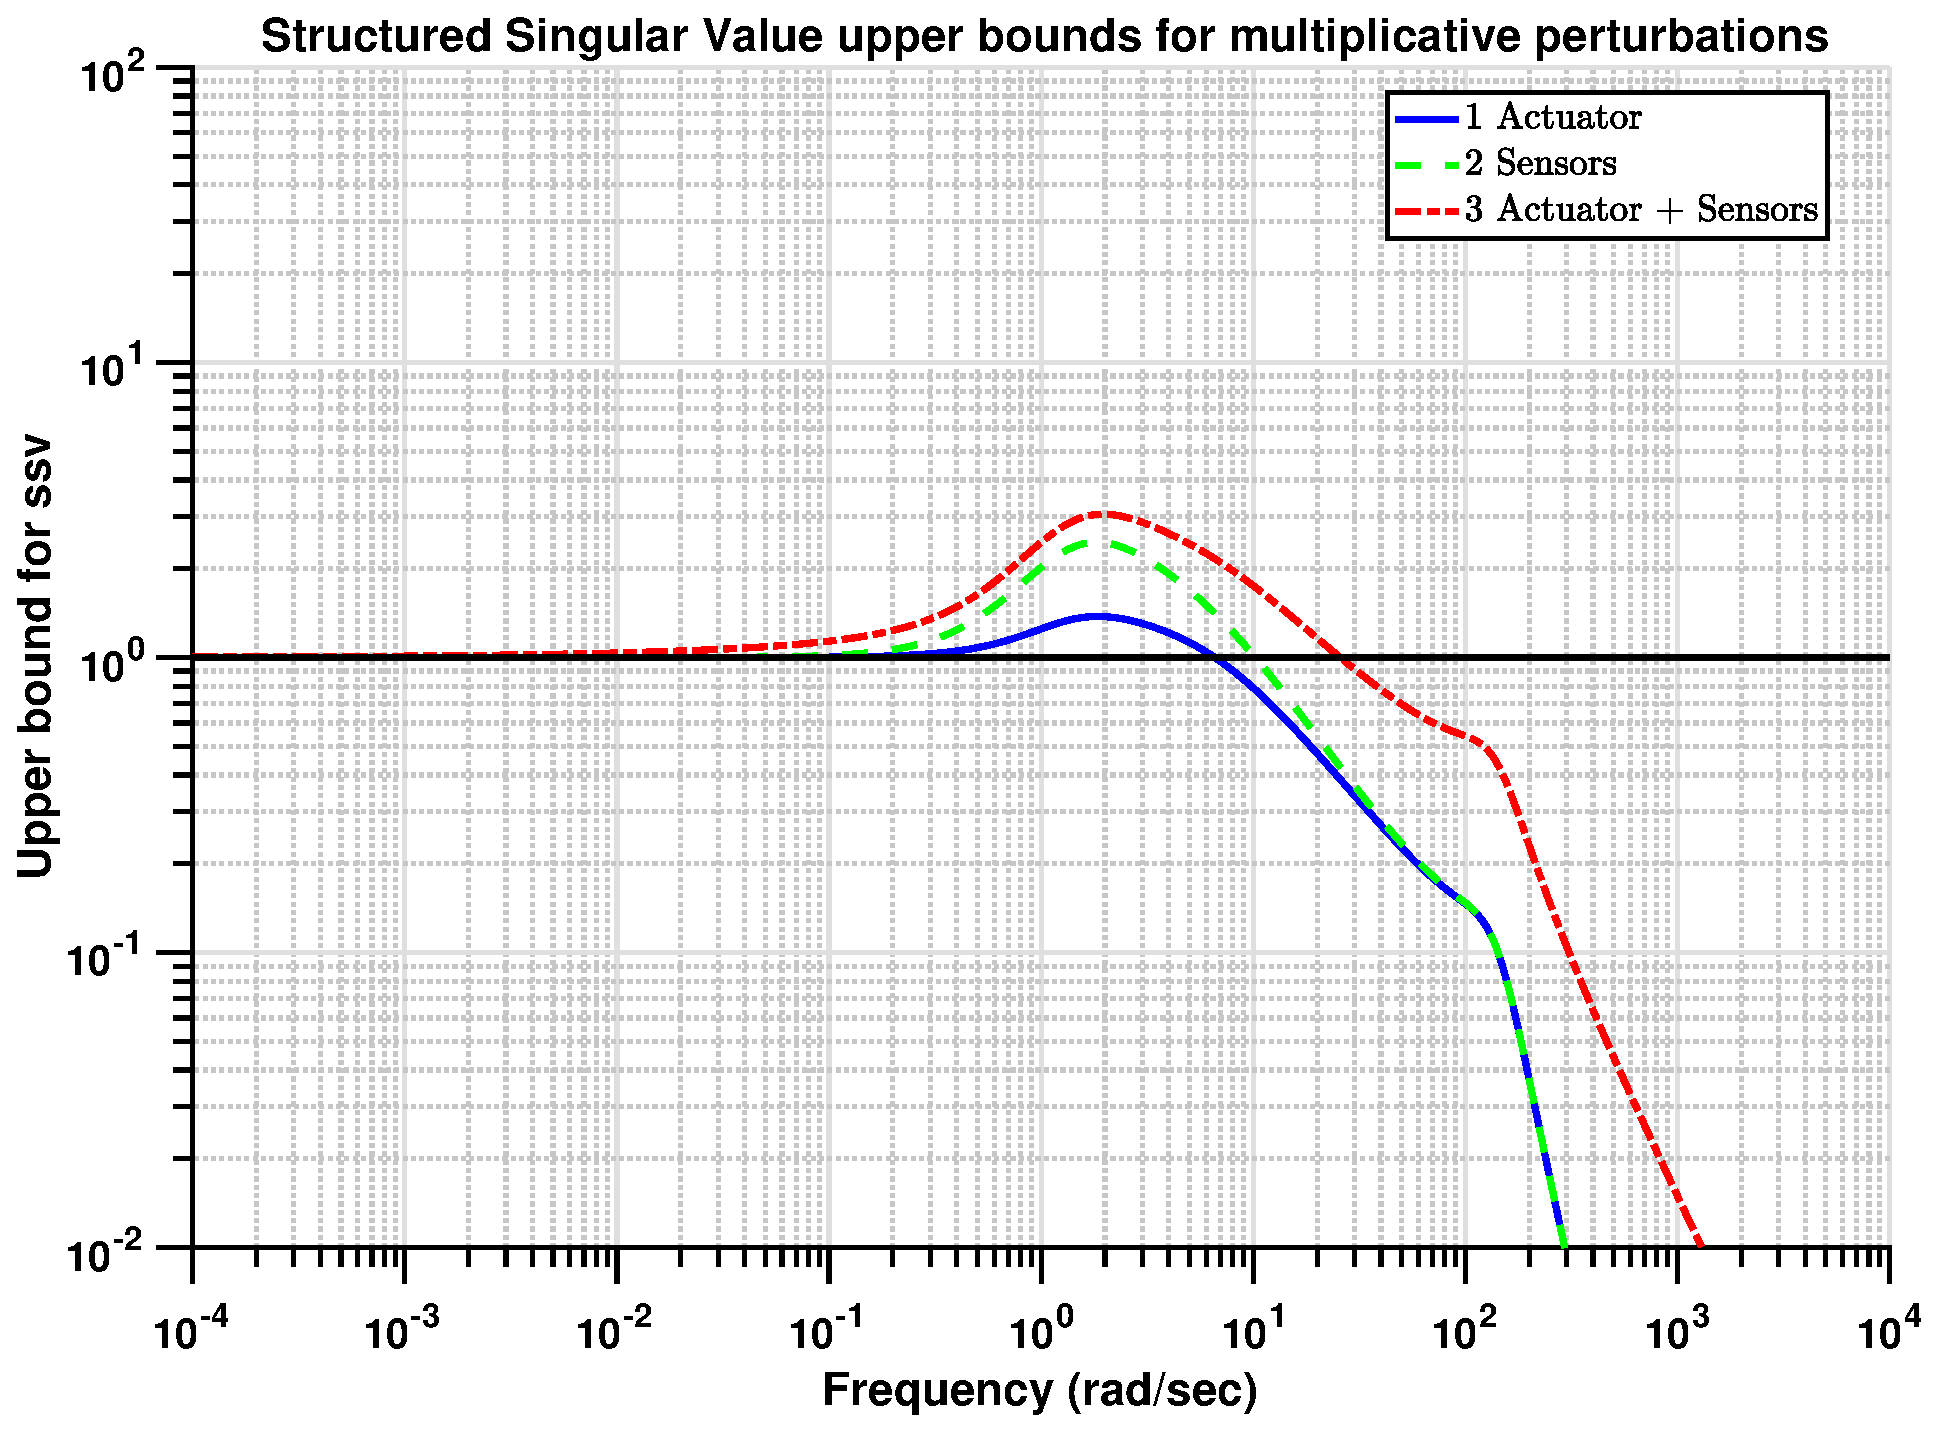
\includegraphics[width=0.9\linewidth]{SSVUpperBNDS}
		\caption{Structured Singular Value Upper Bounds for Sensors and Actuators}
		\label{fig:SSVUpperBNDS}
	\end{figure}
	
	\subsubsection{Uncertainty Blocks}
	For Single-Loop-At-A-Time analysis, the uncertainty configuration considered here is a structured block diagonal consisting of two scalar complex (Transfer Functions) $1\times1$ blocks.
	
	\begin{equation}
	\Delta = \begin{bmatrix}
	\delta_{1} &0\\
	0 & \delta_{2}
	\end{bmatrix}
	\end{equation}
	
	\subsubsection{Single-Loop-At-A-Time Analysis}
	Loops were broken at one actuator and two sensors ($\theta_{PG}$ and $\theta_{RG}$) to find the single-loop-at-a-time (SLAT) loop transfer functions. 
	
	\begin{figure}[H]
		\centering
		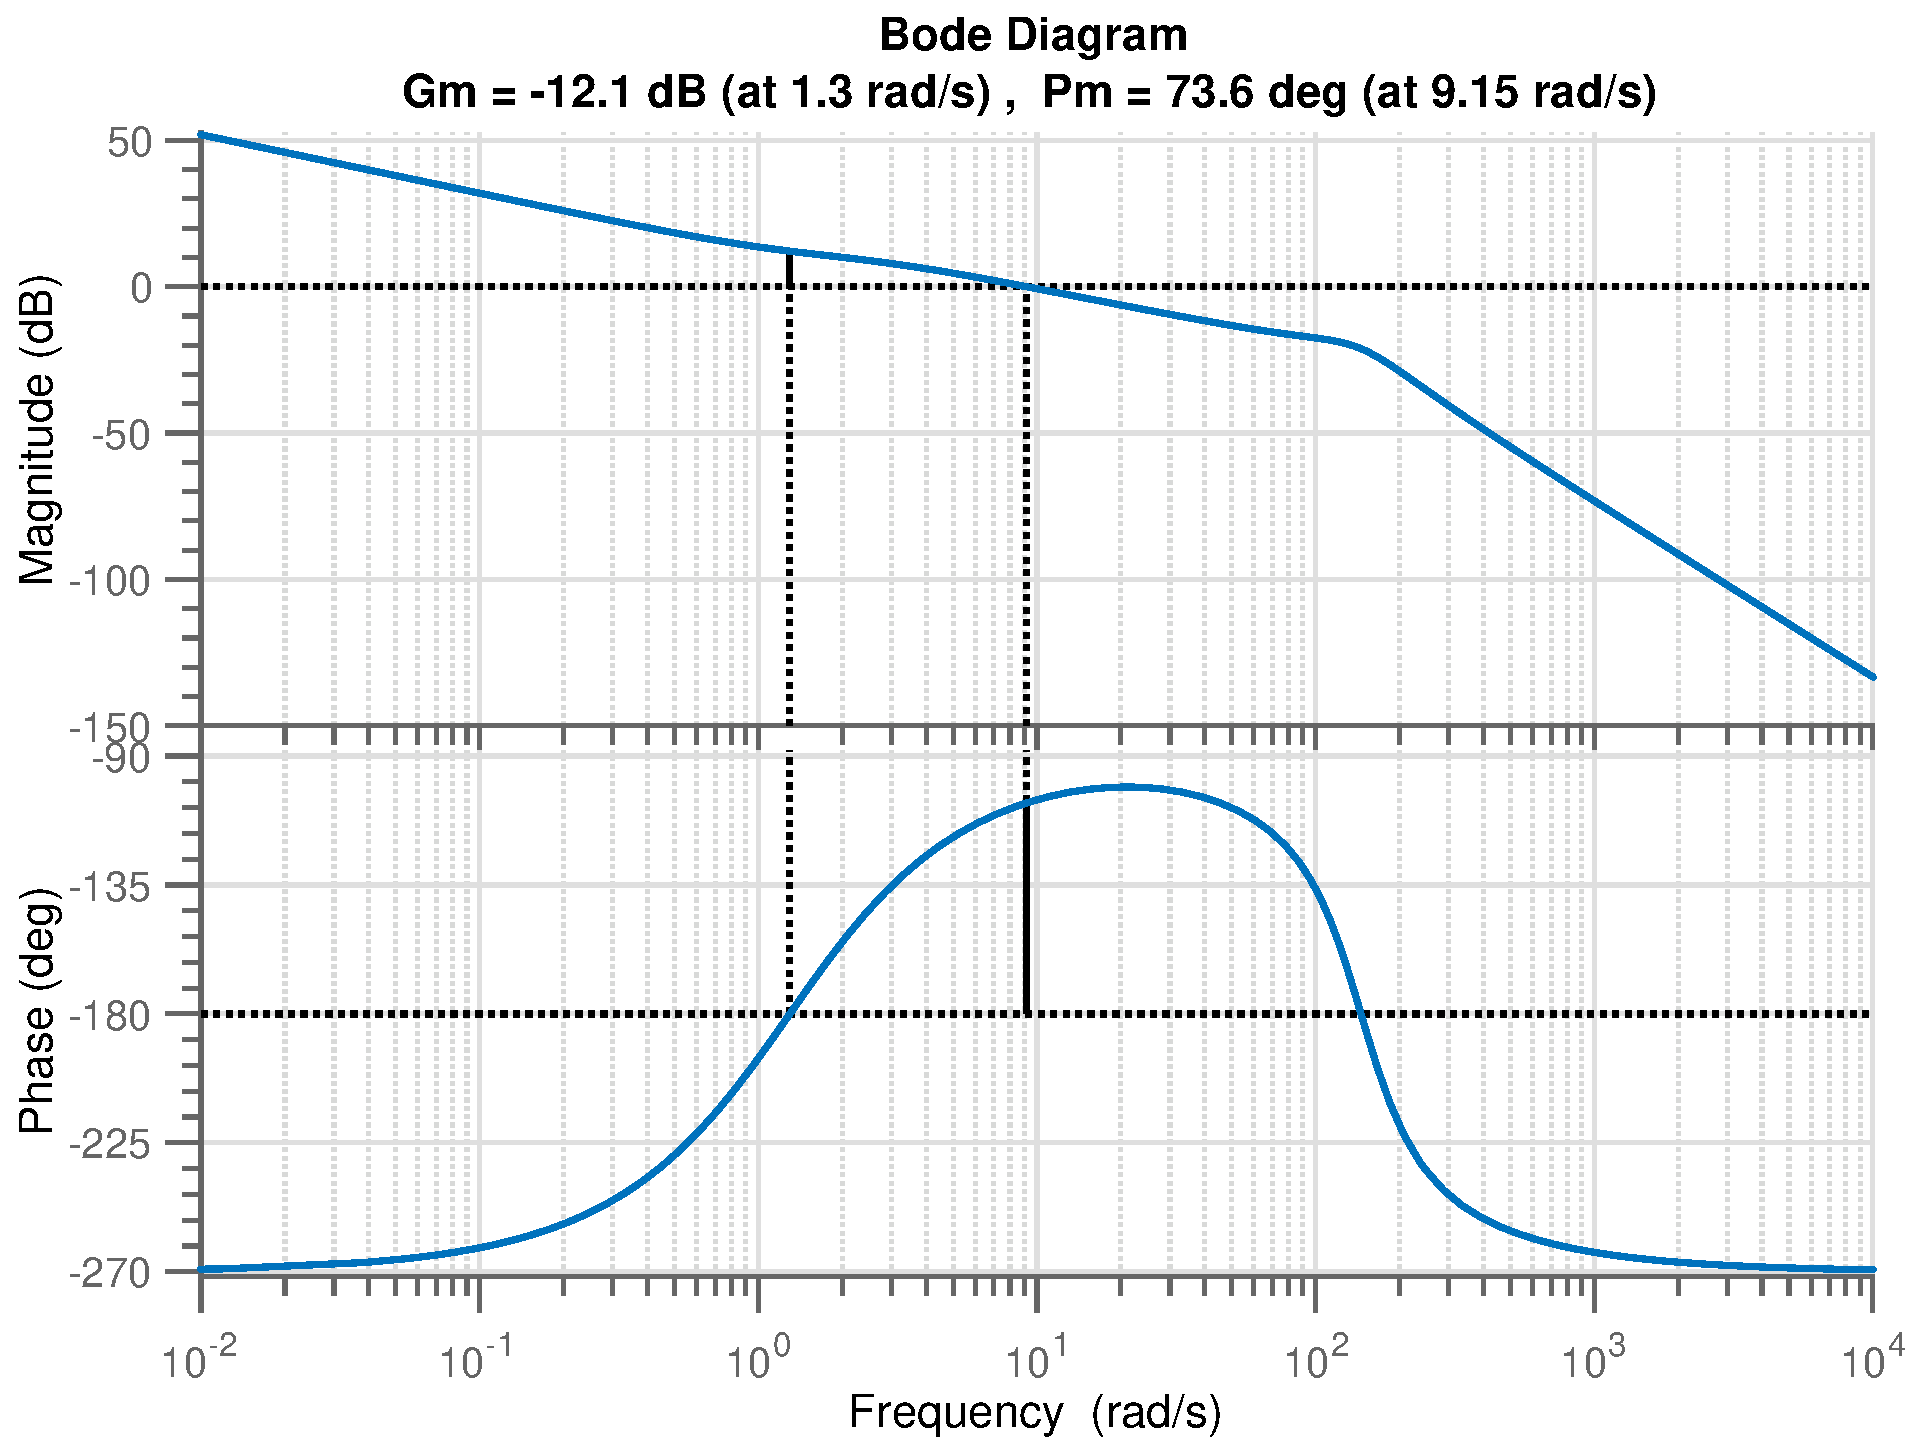
\includegraphics[width=0.8\linewidth]{InputLoopBode_SLAT_U}
		\caption{SLAT Analysis at u}
		\label{fig:inputloopbodeslatu}
	\end{figure}
	
	\begin{figure}[H]
		\centering
		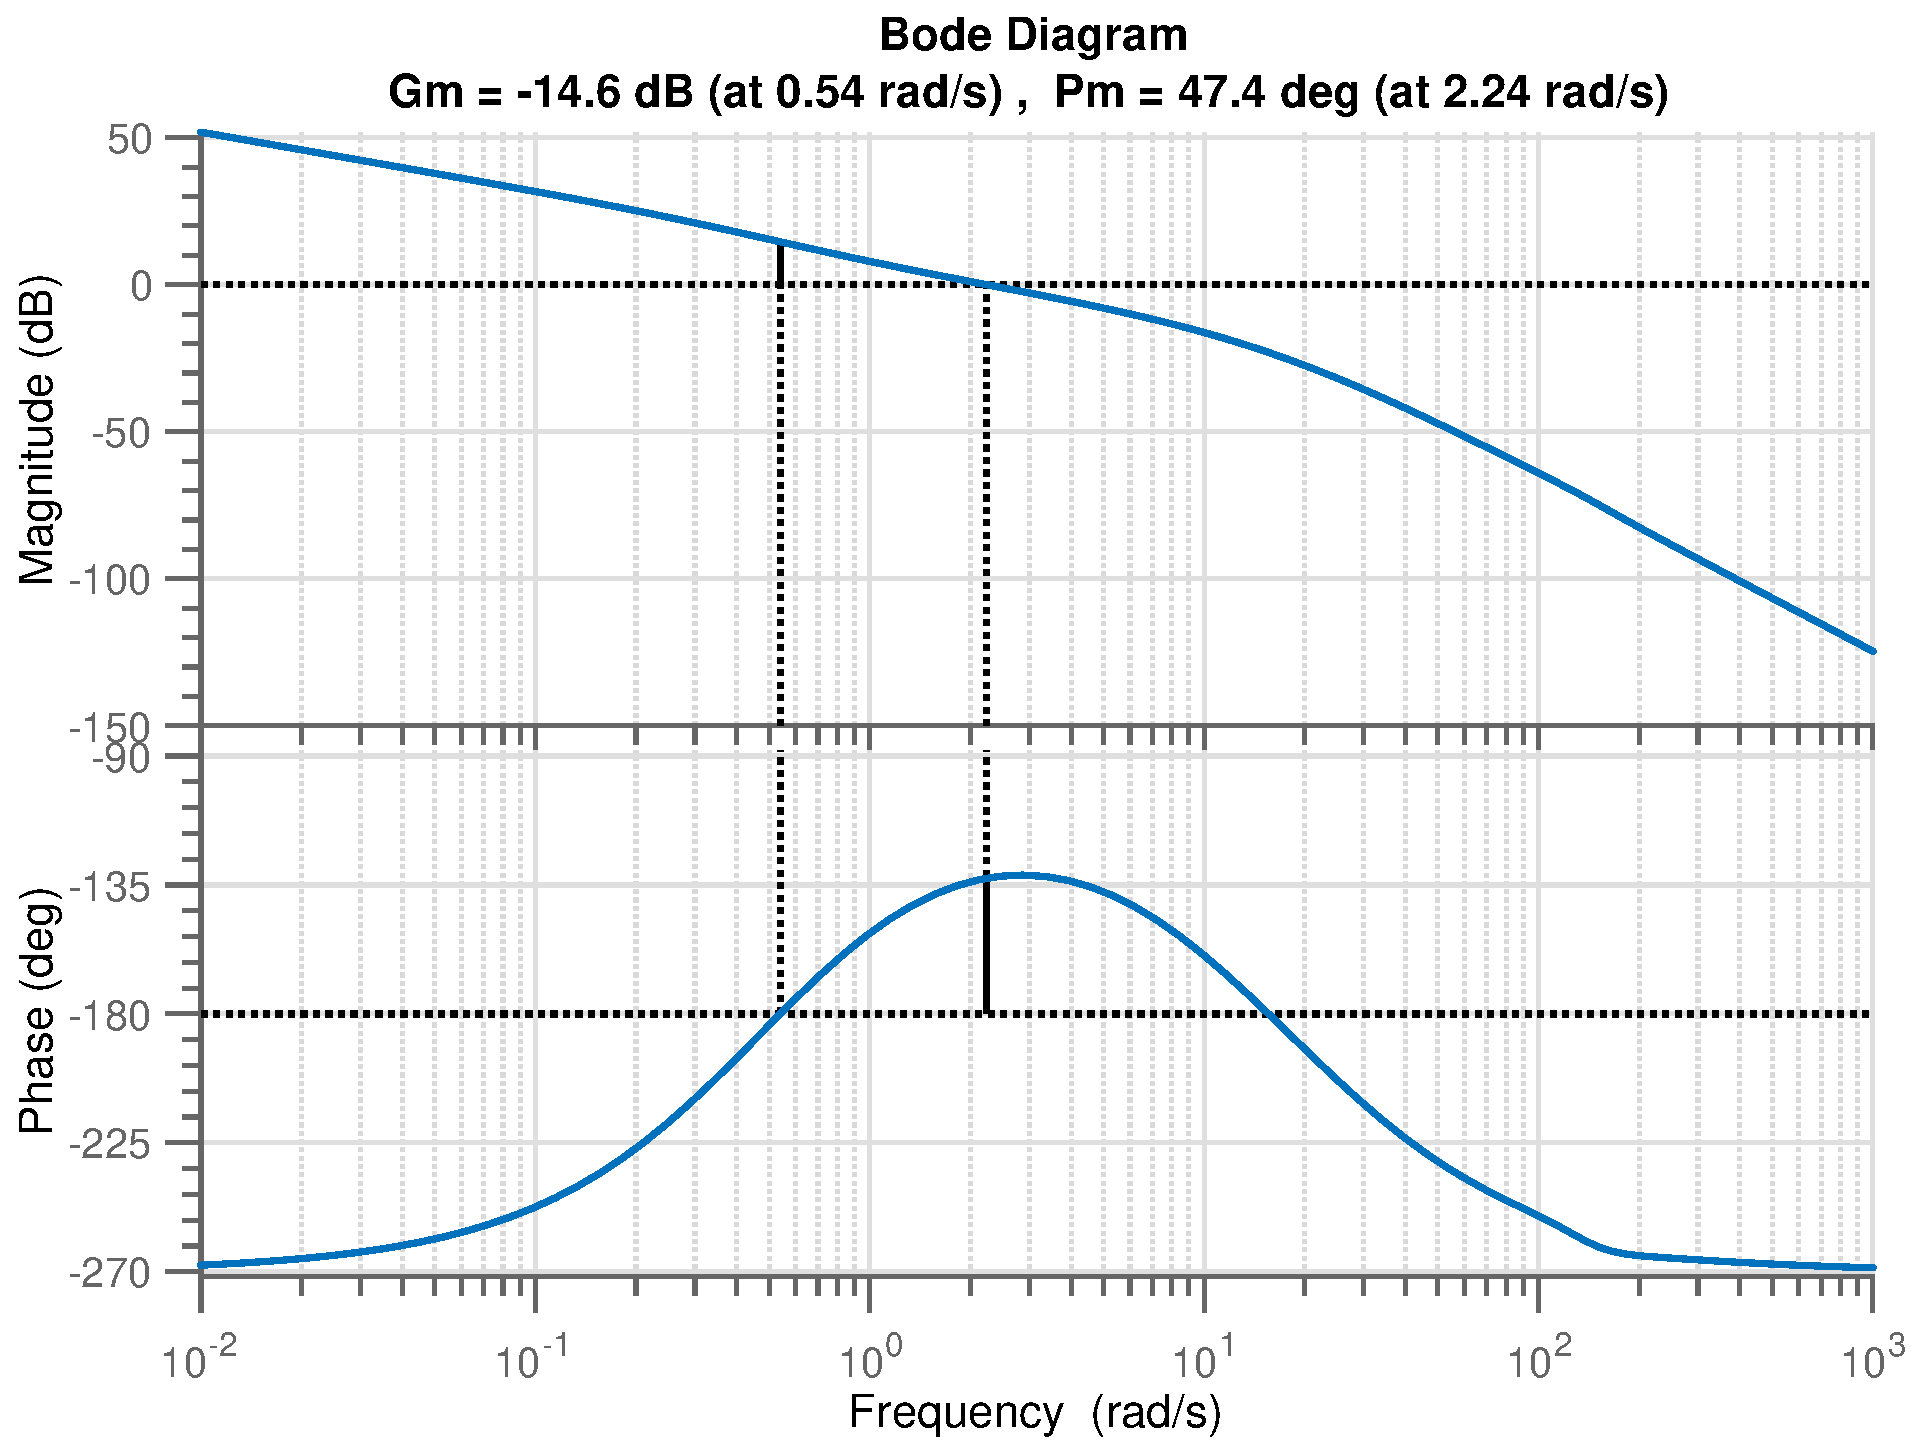
\includegraphics[width=0.8\linewidth]{InputLoopBode_SLAT_Y1}
		\caption{SLAT Analysis at $\theta_{PG}$ measurement}
		\label{fig:inputloopbodeslaty1}
	\end{figure}
	
	\begin{figure}[H]
		\centering
		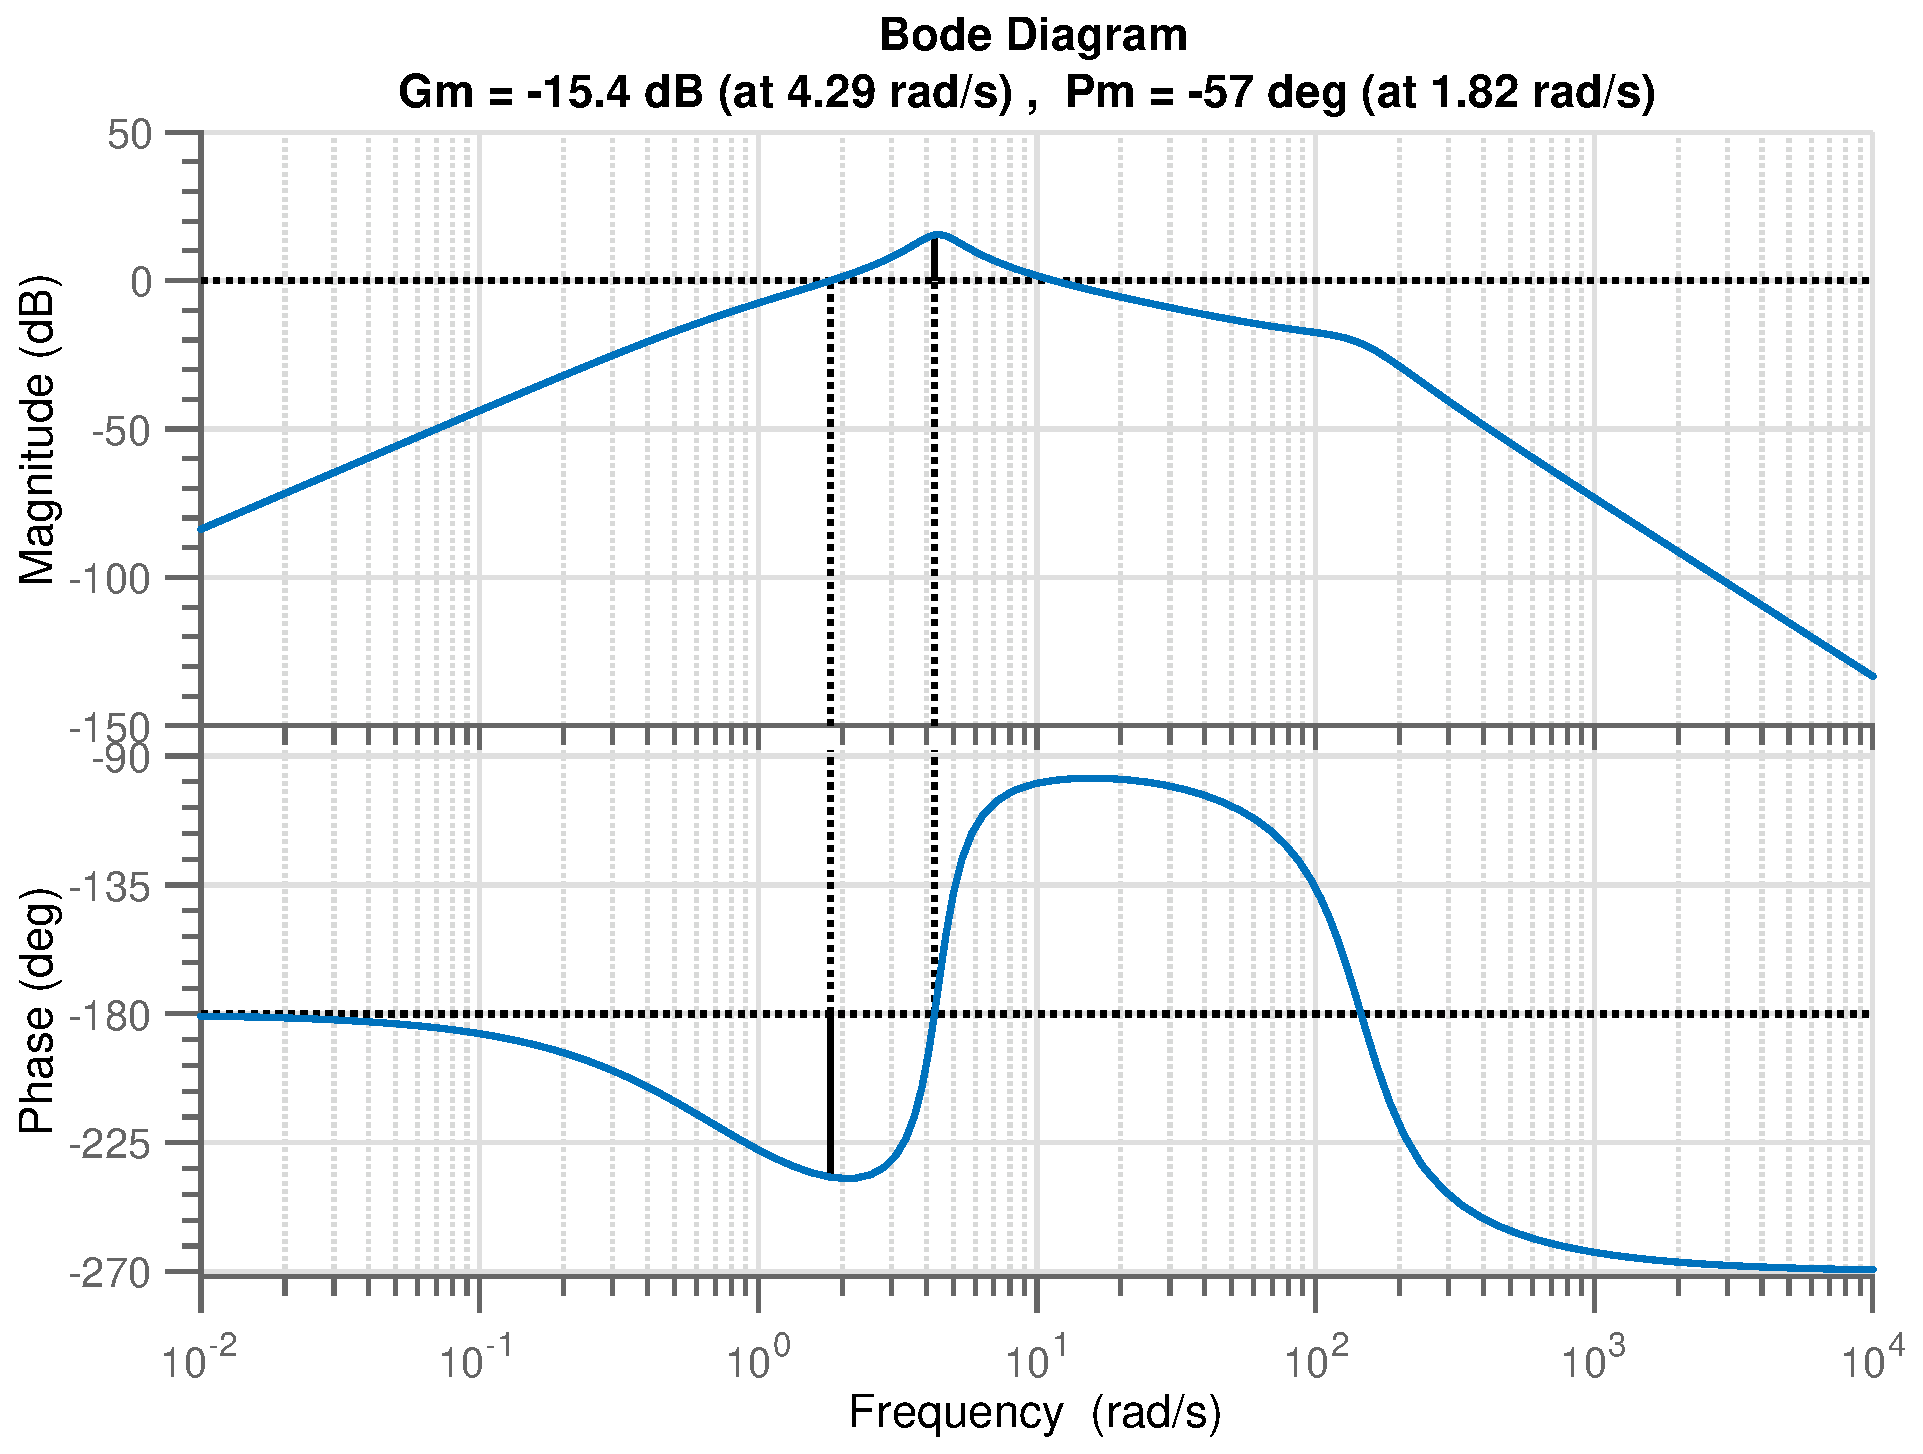
\includegraphics[width=0.8\linewidth]{InputLoopBode_SLAT_Y2}
		\caption{SLAT Analysis at $\theta_{RG}$ measurement}
		\label{fig:inputloopbodeslaty2}
	\end{figure}
	
	\begin{center}
		\begin{tabular}{ |p{3.5cm}|p{2.4cm}|p{2.2cm}|p{2.2cm}|p{2.2cm}|  }
			\hline
			\multicolumn{5}{|c|}{Summary of Single-Loop-At-A-Time Analysis} \\
			\hline
			Loop Broken At & $\omega_{180}$ \texttt{(rad/s)}& GM \texttt{(dB)}& $\omega_c$ \texttt{(rad/s)}& PM \texttt{(deg)} \\
			\hline
			Input $(u)$ & 1.3 & -12.1 & 9.15 & 73.6\\
			& 145 & 21.2 & &\\
			\hline
			Output $(y_1=\theta_{PG})$ & 0.54 & -14.6  & 2.24 & 47.4\\
			& 15.7 & 23.1 & &\\
			\hline
			Output $(y_2=\theta_{RG})$ & 4.29 & -15.4 & 1.82 & -57\\
			& 144 & 21.1 & 11.5 & 81.5\\
			& 0 & $\infty$ & &\\
			\hline
		\end{tabular}
	\end{center}
	
	\noindent The frequency response of SLAT, when the loop was broken at the input is shown in the Figure \ref{fig:inputloopbodeslatu}. Similarly, for first and second output broken loop analysis is shown in the Figure \ref{fig:inputloopbodeslaty1} and \ref{fig:inputloopbodeslaty2} respectively. \texttt{linmod()} was used for obtaining the broken loop transfer functions. 
	
	\begin{itemize}
		\item It is evident that negative phase margin for $\theta_{RG}$ is not as desired but since they are at lower frequency, its not a significant concern. Phase margin frequency is lower than the crossover frequency of the loop. The stability of the loop transfer functions may be a concern due to negative phase margin. 
		\item Overall, all gain margins are found to be greater than 6 dB for either gain increase or gain decrease. In the table, negative gain margin represents gain decrease and positive gain margin represents gain increase margin. 
		\item Moreover, SLAT analysis for $\theta_{RG}$ was considered here because launch vehicles have elastic modes at higher frequencies that were ignored in the modeling. 
		
		
		\begin{equation}
		\label{inq}
		\omega_b^* < \omega_c < 1/\tau
		\end{equation}
		
		\item As mentioned before, $\omega_b^*$ = 1.05 rad/s is a bandwidth frequency specification for desirable performance. $\omega_c$ is a crossover frequency as shown in the table above. $1/\tau$= 25 rad/s is the frequency above which the model is completely unknown/uncertain. Thus, it is verified that the inequality \ref{inq} is satisfied for all the crossover frequencies.
	\end{itemize}
	\subsubsection{Robust Performance}
	
	Robust Performance guarantees stability and satisfactory performance i.e. disturbance rejection property of the control system. The test for SISO robust performance is given by,
	
	\begin{equation}
	\label{eqSISOTest}
	\norm{W_I T_{I}}_{\infty} + \norm{W_P S}_{\infty}< 1 
	\end{equation}
	
	\begin{figure}[H]
		\centering
		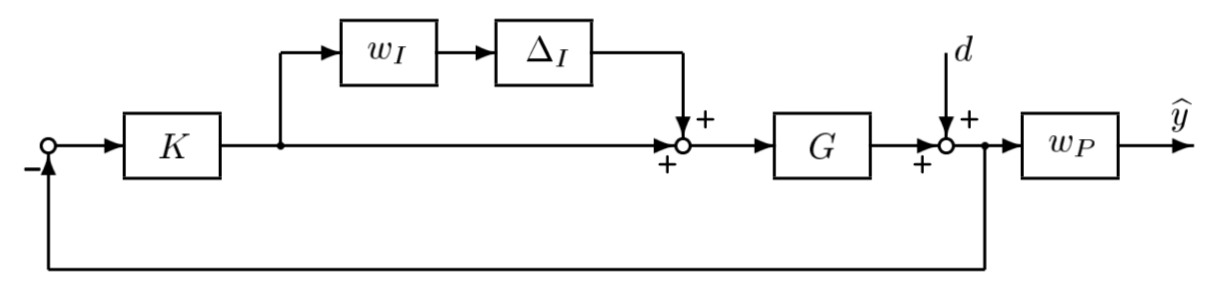
\includegraphics[width=0.8\linewidth]{WIWP}
		\caption{Block diagram for including $W_I$ and $W_p$ as weight matrix}
		\label{fig:wiwp}
	\end{figure}
	
	\begin{figure}[H]
		\centering
		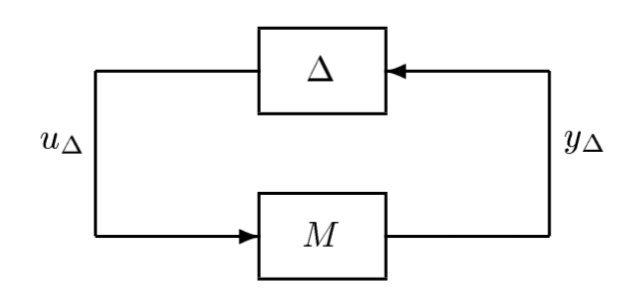
\includegraphics[width=0.4\linewidth]{MD}
		\caption{$M-\Delta$ Architecture}
		\label{fig:md}
	\end{figure}
	
	\noindent As can be seen from attached code, M matrix as shown in Figure \ref{fig:md} can be obtained using Simulink model. For MIMO robust performance, it is desired that $\mu[M] < 1$. For our analysis it is sufficient to check for the SISO test that is presented by inequality \ref{eqSISOTest}. From MATLAB code as attached, $\norm{W_I T_{I}}_{\infty} + \norm{W_P S}_{\infty}$  was found to be 0.9925, i.e. the RP test is satisfied.
	
	\begin{equation}
	\mu[M] = \mu\begin{bmatrix}
	W_p S & W_p G S_I \\
	-W_I S_I K & -W_I T_I
	\end{bmatrix}
	\end{equation}
	
	\section{Summary}
	\noindent In this section, a brief summary on the overall project is provided.
	\begin{itemize}
		\item Open loop plant was analyzed for nominal stability and performance, and found to be unstable, but it was controllable and observable.
		\item In our initial approach, we considered reduced order model that neglected sensor dynamics. Proportional and Integral control was designed for the reduced order model and was implemented on the full $5^{th}$ order model. 
		\item The closed loop system was analyzed for nominal stability and performance. The designed controller was stable and performed well in terms of time domain performance specifications.
		\item Robust stability and performance measures are summarized in the following table. The closed loop was found to be robust stable for the specified perturbation. Figure \ref{fig:summary} shows all the criterion singular values vs. frequency plot.
		\begin{center}
			\begin{tabular}{ |p{4cm}|p{4.8cm}||p{5.2cm}|  }
				\hline
				\multicolumn{3}{|c|}{Summary of Stability and Performance Measures} \\
				\hline
				& Criterion & Results\\
				\hline
				Nominal Stability & Re($\lambda_i$) $<$ 0, $\forall i$  & Satisfied\\
				Nominal Performance & $\norm{W_P S}_{\infty}$ $<$ 1 & $\norm{W_P S}_{\infty}$ = 0.858\\
				Robust Stability & $\norm{W_I T_I}_{\infty}$ $<$ 1  & $\norm{W_I T_I}_{\infty}$ = 0.629\\
				Robust Performance & $\norm{W_I T_{I}}_{\infty} + \norm{W_P S}_{\infty}<$ 1 & $ \norm{W_I T_{I}}_{\infty}+ \norm{W_P S}_{\infty}$ = 0.993\\
				\hline
			\end{tabular}
		\end{center}
		
		\item The designed controller works well for vehicles with bending mode frequency at least 25 rad/s. Lower bending mode frequencies will conflict with the assumption that was made. Potentially, controller has to be redesigned for such consideration. 
		
		\begin{figure}[H]
			\centering
			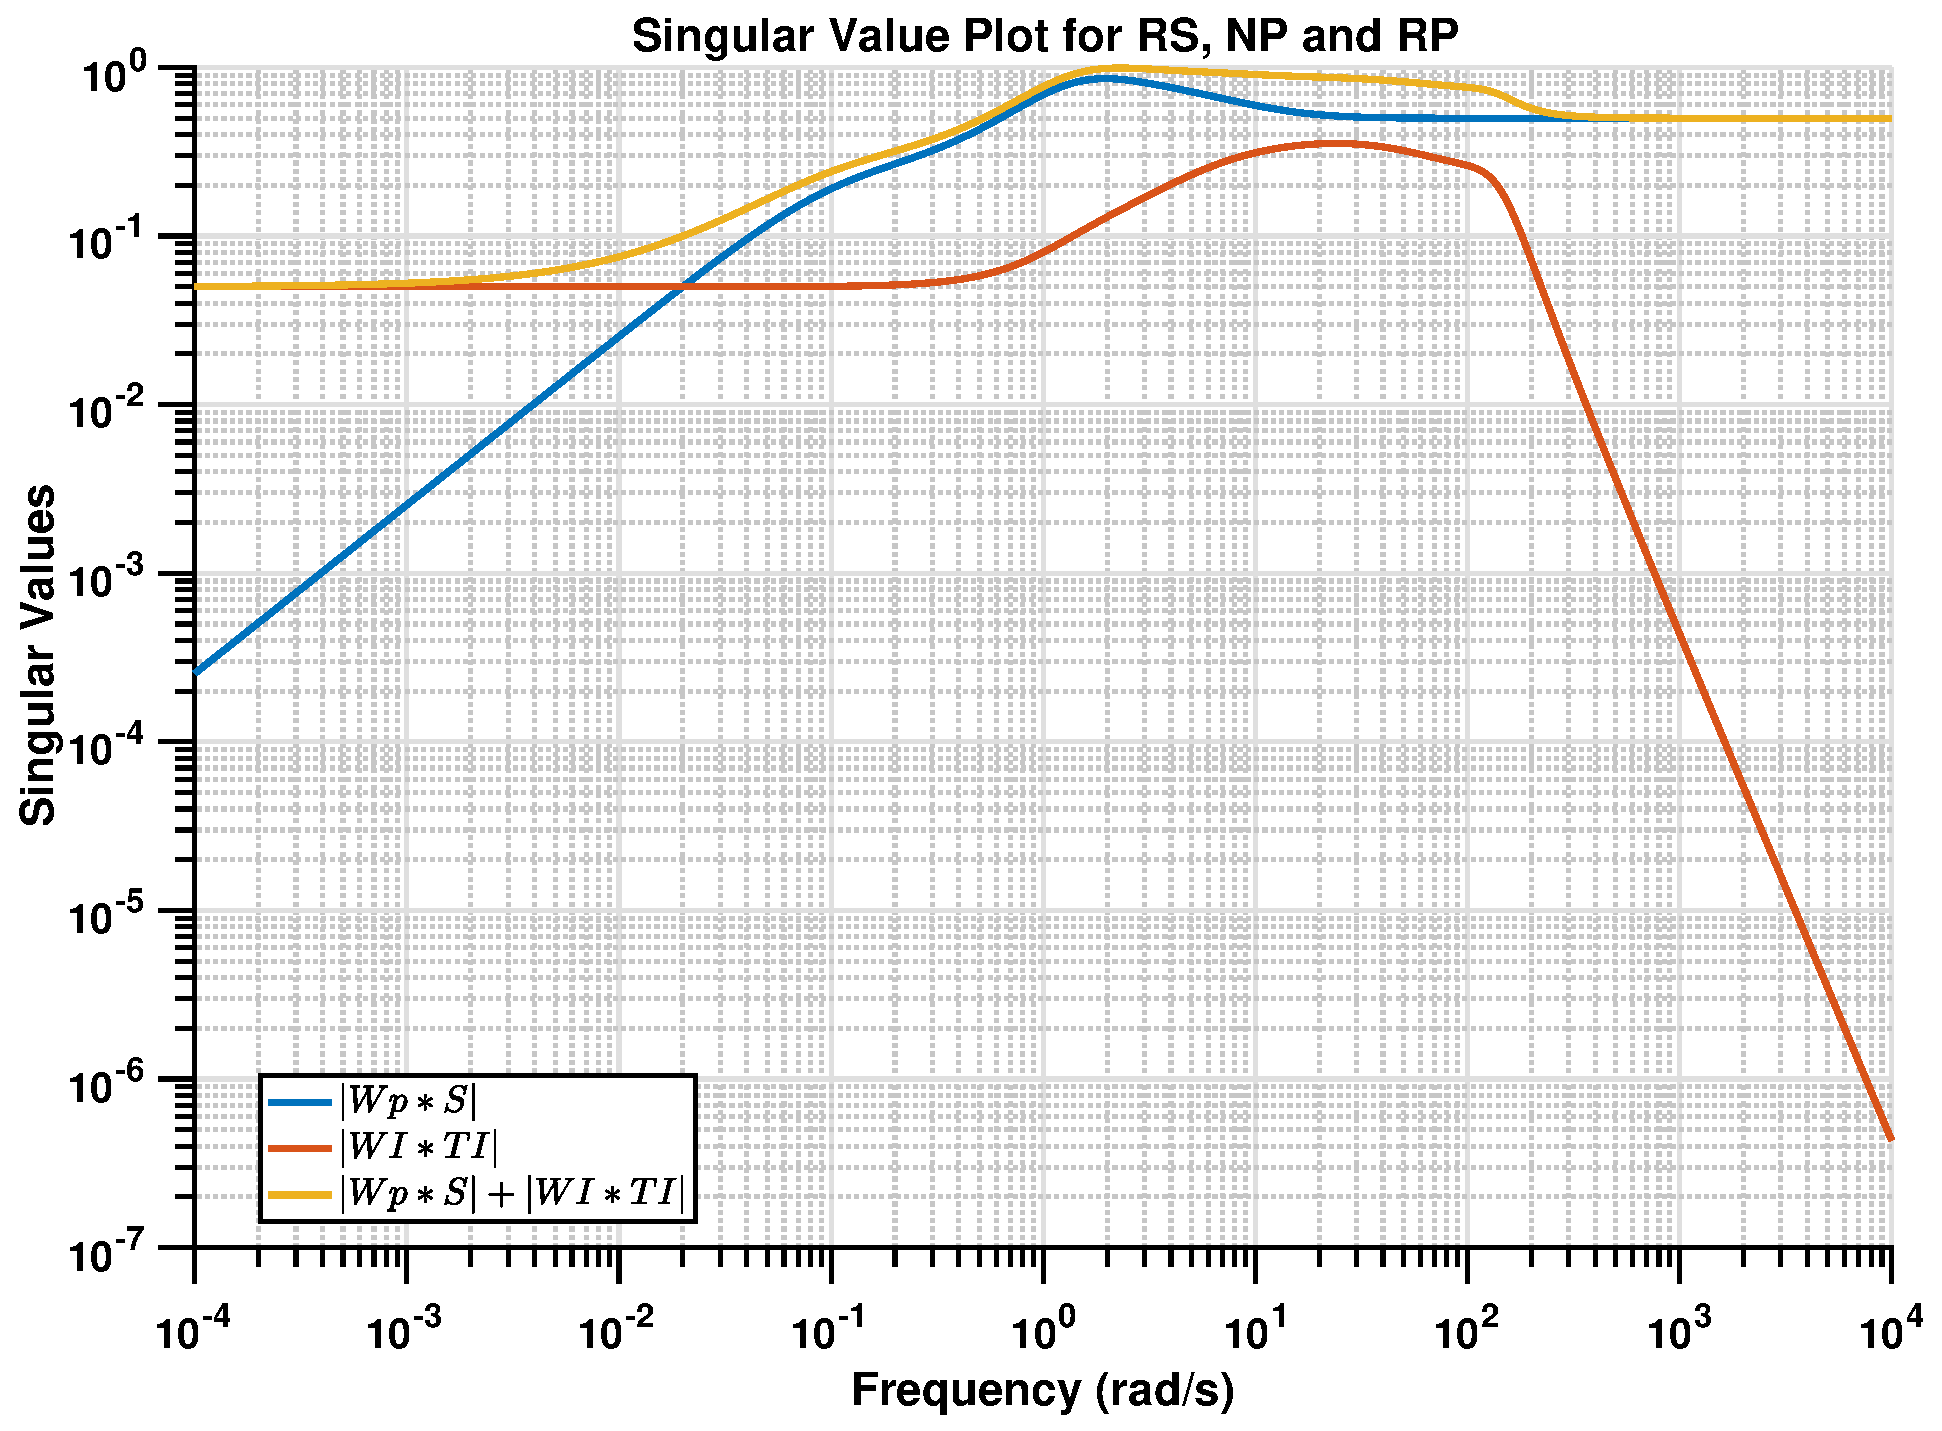
\includegraphics[width=0.9\linewidth]{Summary}
			\caption{RS, NP and RP Summary}
			\label{fig:summary}
		\end{figure}
	\end{itemize}
	
	\section*{Conclusion}
	Control design for the launch vehicle attitude has been studied in this work. Linearized Time Invariant dynamics of Rocket system were used to design an attitude control system using classical and modern control concepts. It was identified that PI feedback compensator can deliver the desired control behavior and performance for this system. Nominal Performance, Nominal Stability, Robust Performance and Robust Stability were analyzed using MATLAB and Simulink tools. It was realized that the controller performance depends on the certain assumptions that were made during the design of a controller. Furthermore, the trade-off between desirable performance at lower frequency and potential compromise at higher frequency was realized during the project. Overall, this was a very good learning experience which allowed us to apply the knowledge that we learned during class. 
	
	\section*{Acknowledgment}
	Our sincere thanks to Prof. Dale Enns for his valuable knowledge, guidance and patience during this project. His classroom discussions and suggestions through email were very helpful for the completion of the project.
	
\begin{thebibliography}{9}
	\bibitem{cite1} Kim, C. H., Commercial Satellite Launch Vehicle Attitude Control Systems Design and Analysis (H-infinity, Loop Shaping, and Coprime Approach): H-infinity, Loop Shaping, and Coprime Factorization Approach, 2007
	
	\bibitem{cite2} Greensite, A.L., Analysis and design of space vehicle flight control systems, volume 2. National aeronautics and space administration, 1967
	
	\bibitem{cite3} Skogestad, S. and Postlethwaite, I., 2007. Multivariable feedback control: analysis and design (Vol. 2, pp. 359-368). New York: Wiley
\end{thebibliography}
	
	\appendix
	\section{Simulink Model Block Diagram}
	%\begin{itemize}
	%	\item Proportional \& Integral Control Simulink Model 
	%\end{itemize}
	\section{MATLAB Published Code}
	\label{appendix}
	%\begin{itemize}
	%	\item Nominal Stability \& Nominal Performance (Open Loop and Closed Loop)
	%\end{itemize}
	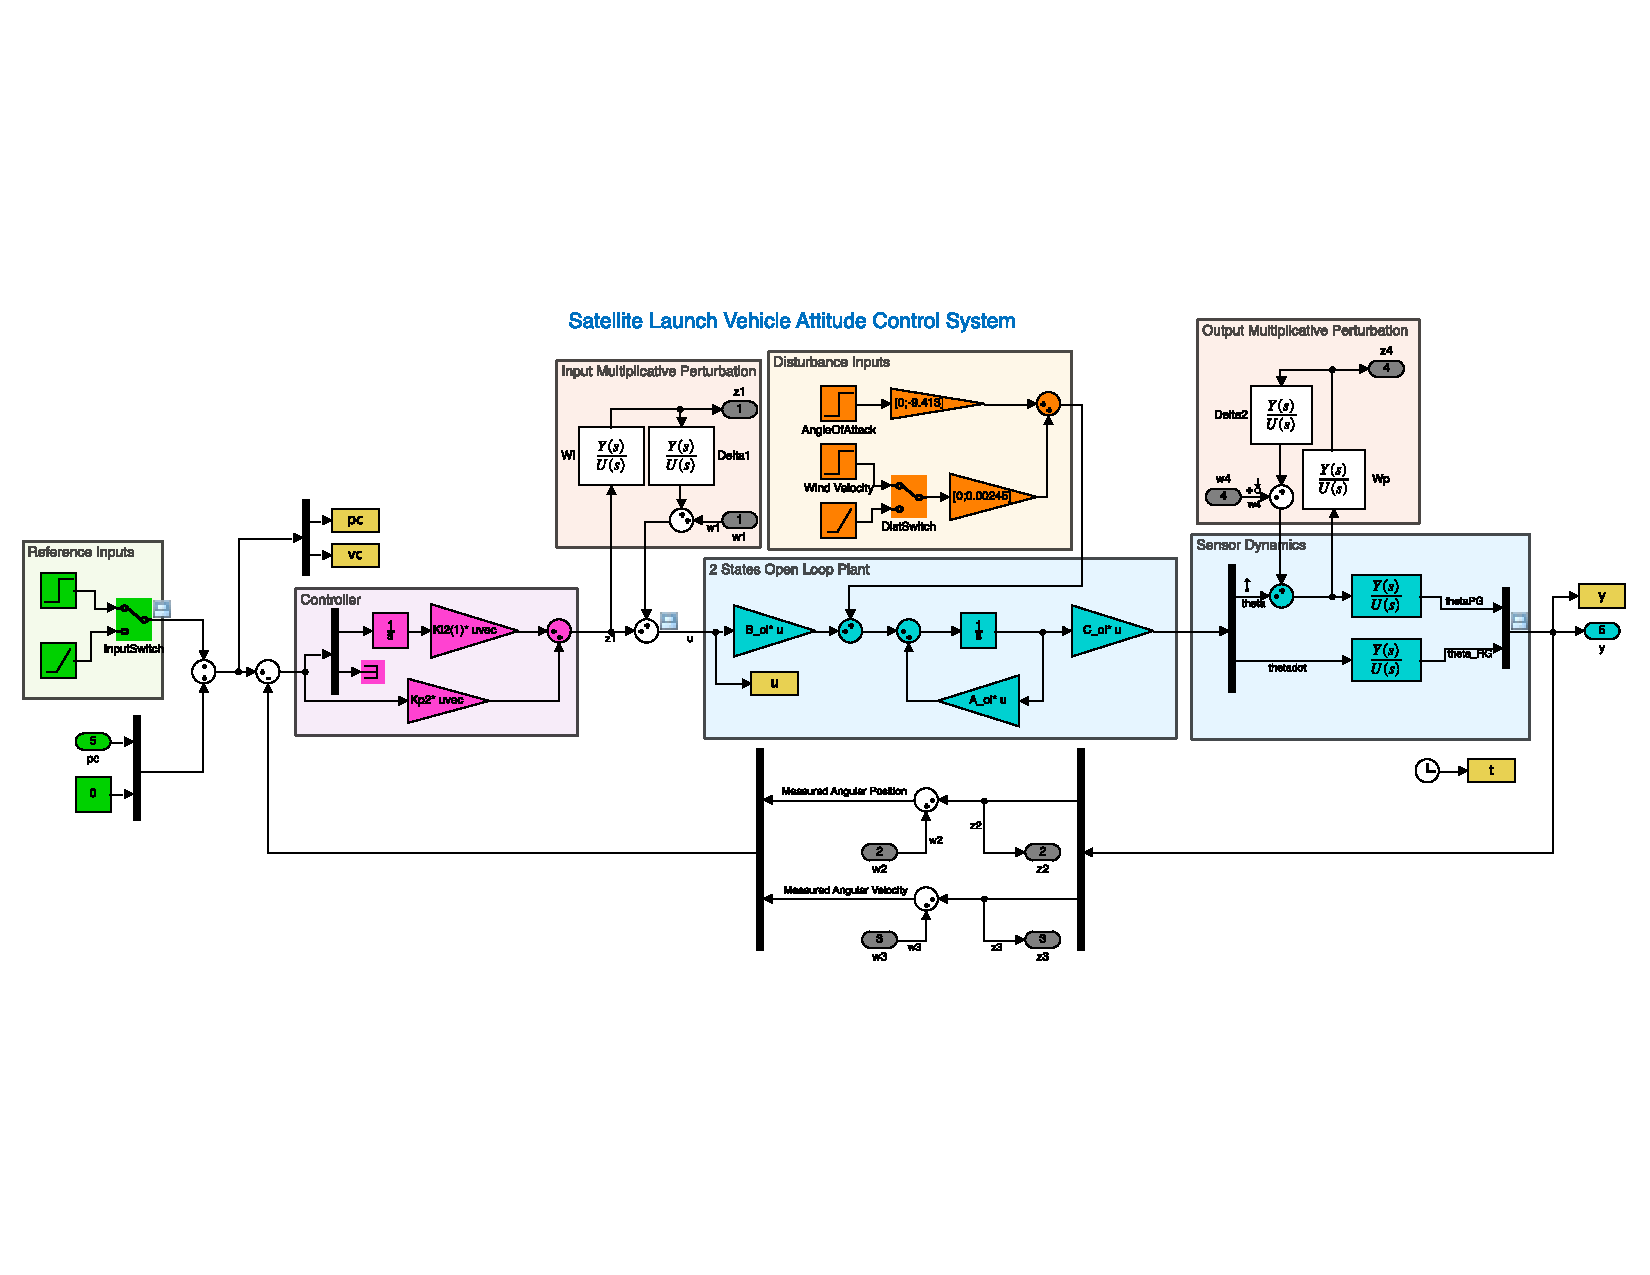
\includepdf[pages=-]{LaunchVehicle.pdf}
	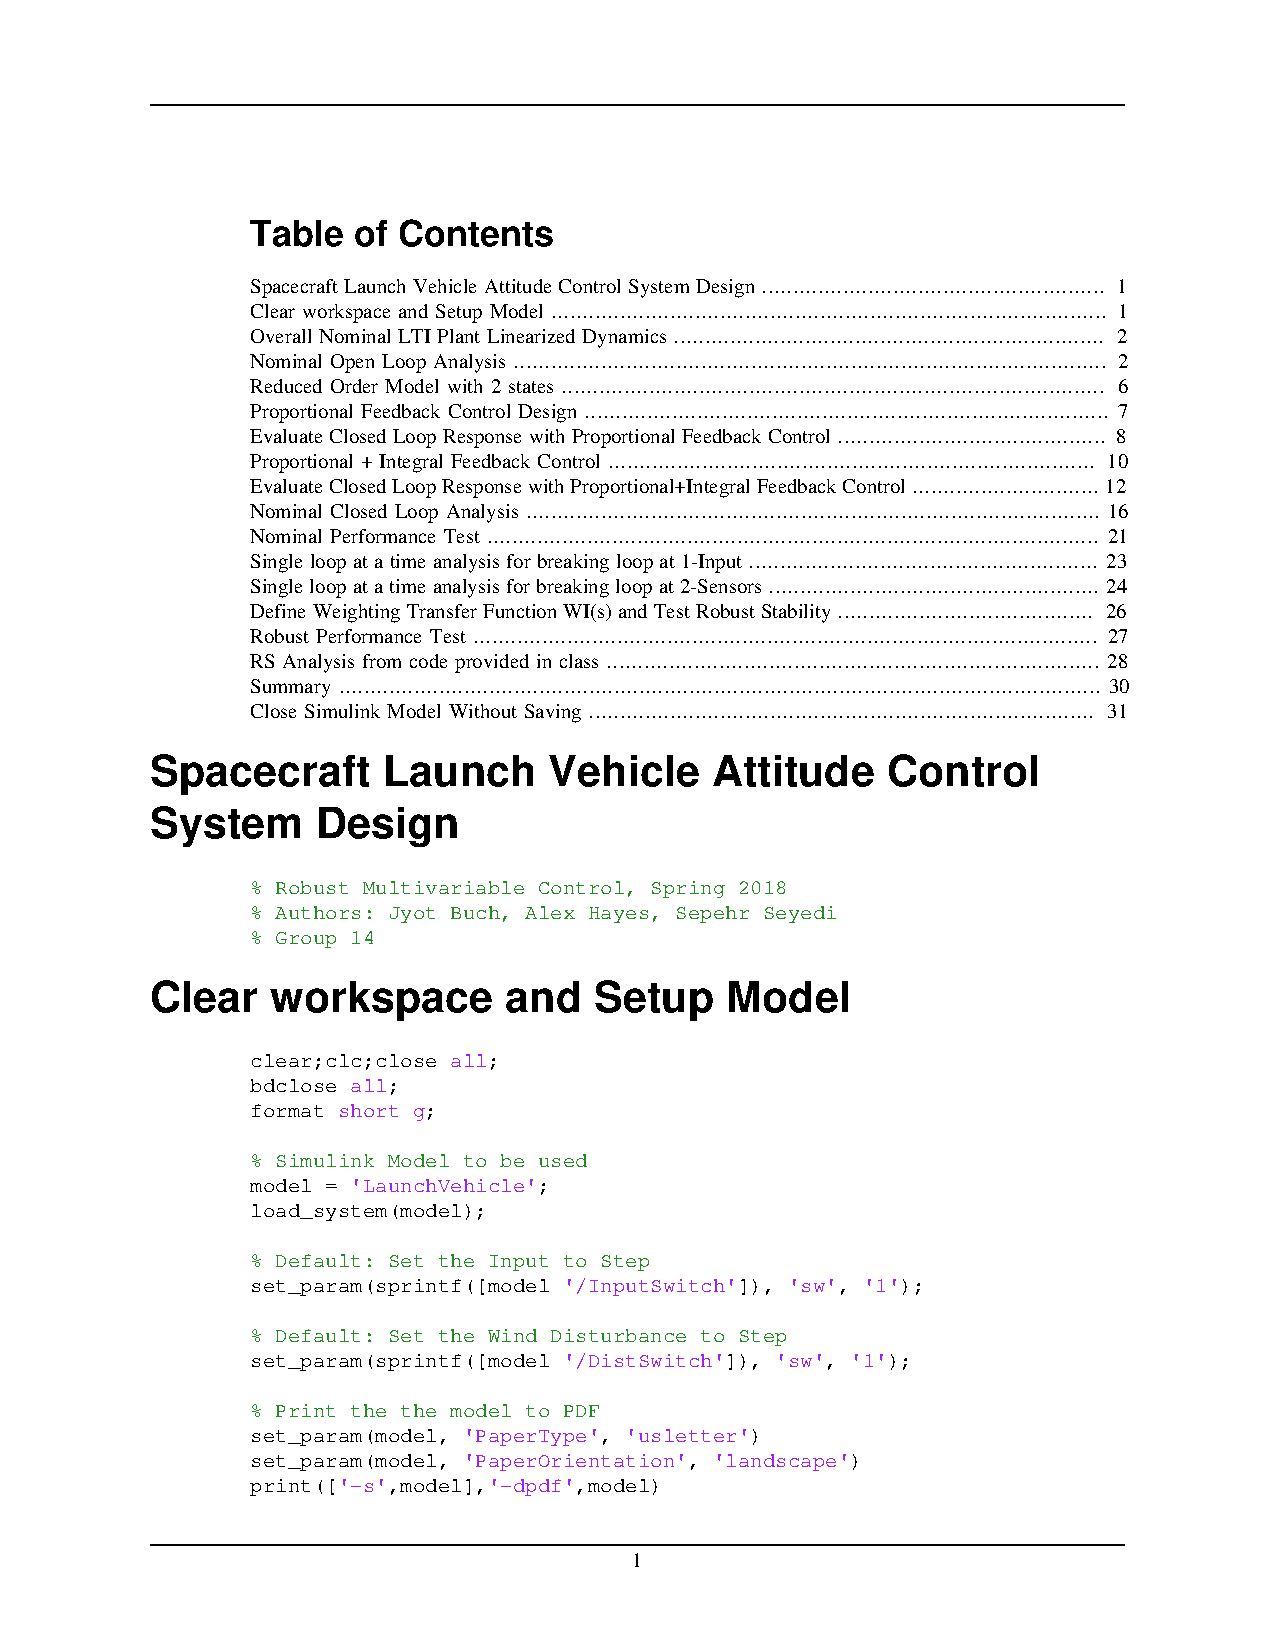
\includepdf[pages=-]{main.pdf}
\end{document}



















